\documentclass[11pt, spanish]{book}
\usepackage{tocbibind}
\usepackage[colorlinks=true, linkcolor=linkblue, citecolor=linkblue]{hyperref}
\usepackage[spanish]{babel}
\usepackage[utf8]{inputenc}
\usepackage[svgnames]{xcolor}
\usepackage{ellipsis}
\usepackage{graphicx}
\usepackage{caption}
\usepackage{subcaption}
\usepackage{afterpage}
\usepackage{float}
\usepackage{here}
\usepackage{color}
\usepackage{ragged2e}
\usepackage{geometry}
\usepackage{makeidx}
\usepackage{microtype}
\usepackage{booktabs}
\usepackage[svgnames]{xcolor}
  \definecolor{diffstart}{named}{Grey}
  \definecolor{diffincl}{named}{Green}
  \definecolor{diffrem}{named}{Red}

\usepackage[table]{xcolor}


\usepackage{listings}
  \lstdefinelanguage{diff}{
    basicstyle=\ttfamily\small,
    morecomment=[f][\color{diffstart}]{@@},
    morecomment=[f][\color{diffincl}]{+\ },
    morecomment=[f][\color{diffrem}]{-\ },
  }

\makeindex

\pagestyle{headings}

\definecolor{dkgreen}{rgb}{0,0.6,0}
\definecolor{gray}{rgb}{0.5,0.5,0.5}
\definecolor{mauve}{rgb}{0.58,0,0.82}
\definecolor{linkblue}{RGB}{18,18,115}

\geometry{top=3cm, bottom=3cm}
\textheight=21cm
\textwidth=17cm
% \topmargin=1cm
\oddsidemargin=0cm
\parindent=3mm
\pagestyle{plain}
\setlength{\parskip}{0.5em}

\renewcommand{\arraystretch}{1.5}
\setlength{\tabcolsep}{10pt}
\renewcommand{\tablename}{Tabla}

\begin{document}
\begin{titlepage}
    \begin{center}
        \vspace*{1cm}

        \begin{figure}
            \centering
            \begin{minipage}[t]{0.45\textwidth}\centering%
                
\includegraphics[width=\textwidth]{LogoUNC.jpeg}
            \end{minipage}\hfill
            \begin{minipage}[t]{0.45\textwidth}\centering%
                
\includegraphics[width=\textwidth]{LogoFCEFyN.png}
            \end{minipage}
        \end{figure}

        \Huge
        \textbf{Modelado del planificador a corto plazo con redes de Petri}

        \vspace{1.5cm}

        \Large
        \textbf{Autores:} Leandro Agustin Drudi, Nicolás Goldman
        \vspace{.5cm}

        \large
        10 de diciembre de 2022
        \vspace{1cm}

        \normalsize
        \textbf{Email:} drudilea@gmail.com, nicolasgoldman07@gmail.com
        \vspace{.5cm}

        \textbf{Teléfonos:} (351)5307196, (3547)560104
        \vspace{.5cm}

        \textbf{Legajos:} 40.245.918, 40.416.606
        \vspace{1.5cm}

        \textbf{Director:} Maximiliano Eschoyez
        \vspace{.5cm}

        \textbf{Co-Director:} Nicolás Papp
        \vspace{1cm}

        \vspace{0.5cm}

        \vfill

    \end{center}
\end{titlepage}
\thispagestyle{empty}

% Para numerar en romanos
\frontmatter

\begin{Large}
    \textbf{Resumen}
    \vspace{.5cm}
\end{Large}

El sistema operativo se encarga de gestionar los recursos de hardware de un dispositivo electrónico y de brindar servicios a los programas de aplicación. La gestión de los procesos e hilos y los recursos de un sistema operativo son fundamentales para su correcto funcionamiento y desempeño. En este contexto, la planificación es una tarea crítica para asegurar el uso eficiente de los recursos del sistema.\par

Este trabajo parte de un proyecto integrador previo desarrollado por dos alumnos de la FCEFyN, que realizaron un modelado y optimización del planificador de corto plazo mediante Redes de Petri. Las Redes de Petri son una herramienta matemática formal de modelado que permite representar y analizar sistemas de eventos discretos, como es el caso de la planificación de procesos. El uso de ellas, nos permitirá comprobar con mayor facilidad la ausencia de problemas de concurrencia muy comunes en la planificación, así como también aportarán a la hora de captar los estados y eventos del planificador.\par

En el marco de esta investigación, comenzamos con la adaptación del proyecto integrador previo a la última versión del sistema operativo. La actualización del proyecto no solo nos brinda acceso a nuevas funcionalidades avanzadas, sino que también nos permite aprovechar las mejoras en términos de seguridad implementadas en dicha versión. Además, las versiones anteriores eventualmente dejan de tener soporte por parte de la comunidad, dificultando la colaboración y el intercambio de conocimientos.\par

Planteadas las actualizaciones correspondientes, se abordan dos aspectos cruciales en la optimización de la gestión de recursos en sistemas operativos. En primer lugar, se examina el ``Encendido y Apagado de Procesadores'' como un primer paso en la implementación de soluciones de ahorro de energía a nivel de software, antes de considerar enfoques de hardware. La finalidad es permitir la gestión activa de la energía al apagar procesadores no utilizados, lo que conlleva a una reducción significativa en el consumo energético, contribuyendo a una mayor eficiencia operativa del sistema. En segundo lugar, se introduce el concepto de ``Monopolización de Núcleos'' como una estrategia para priorizar procesos críticos por sobre otros, minimizando así interrupciones no deseadas. La capacidad de asignar núcleos específicos a tareas es fundamental para garantizar un rendimiento consistente y predecible en diversos entornos. \par

\tableofcontents
\listoffigures
\listoftables

% Reinicia contador de páginas y numera en arábigo
\mainmatter

\section{Introducción}
La planificación a corto plazo de un sistema operativo es la parte del sistema que se encarga de tomar decisiones sobre qué tareas se deben ejecutar y en qué orden. El objetivo principal de la misma es hacer un uso eficiente de los recursos de CPU disponibles y minimizar el tiempo de respuesta de los procesos.\par

El sistema operativo elegido para realizar este proyecto y las modificaciones pertinentes, es FreeBSD.\@ Éste es un sistema operativo libre y de código abierto, basado en Unix, que se utiliza principalmente en servidores y estaciones de trabajo. Es conocido por su escalabilidad y robustez, así como por su capacidad de adaptarse y personalizarse según las necesidades del usuario.\par


El planificador de bajo nivel se ejecuta cada vez que un hilo se bloquea o interrumpe, y se debe seleccionar un nuevo hilo para ejecutar. Para ser eficiente, al ejecutarse miles de veces por segundo, debe tomar decisiones rápidamente con la menor cantidad de información posible. Para simplificar su tarea, el kernel mantiene un conjunto de colas de ejecución para cada CPU.\@ Cuando una tarea se bloquea en una CPU, la responsabilidad del planificador de bajo nivel es encontrar y elegir el hilo con la máxima prioridad en la cola de ejecución asignada a esa CPU.\par

Este trabajo se construye sobre los cimientos establecidos en un proyecto integrador previo, donde se abordó la mejora del scheduler en el sistema operativo FreeBSD.\@ En dicha investigación, se identificó la naturaleza estadística del proceso de asignación de tiempo de procesador y se propuso un modelo basado en redes de Petri para introducir determinismo y reducir la incertidumbre en la toma de decisiones. En este proyecto, buscamos sumarnos a esta trayectoria, aprovechando los conocimientos adquiridos para abordar nuevas dimensiones en la optimización de la gestión de recursos en sistemas operativos.\par

\subsection{Oportunidad}
El proyecto integrador previo estableció una base sólida para la comprensión integral del funcionamiento de los sistemas operativos y demostró la relevancia de la planificación en el rendimiento del sistema. Este logro requirió un compromiso considerable y una laboriosa inversión de tiempo en la construcción de modelos, así como en el análisis de los resultados obtenidos.\par

No obstante, dada la continua evolución tecnológica y la evolución de las necesidades de los usuarios, se hace imperativo mantener una constante actualización y refinamiento de dicha implementación.\par

En este contexto, la presente oportunidad de trabajo se centra en la incorporación de nuevas funcionalidades y mejoras al planificador a corto plazo del sistema operativo. El objetivo principal radica en alcanzar niveles superiores de eficiencia y desempeño en las operaciones que se ejecutan en el sistema. Para ello, aprovecharemos el conocimiento y las ventajas que ofrecen las Redes de Petri, herramientas que nos permitirán introducir innovaciones de manera efectiva, al tiempo que conservamos las características fundamentales del sistema base.\par


\subsection{Motivación}
La investigación previa en el área de la planificación a corto plazo de sistemas operativos, permitió encontrar una solución efectiva para reducir el indeterminismo en este tipo de sistemas. En concreto, la implementación del planificador a corto plazo de FreeBSD utilizando Redes de Petri, ha demostrado muchas ventajas mediante esta técnica de modelado.\par

Por otro lado, la administración eficiente de la energía es un tema de interés en la actualidad, debido al aumento de la demanda de energía y al impacto ambiental. En este sentido, el uso de técnicas de ahorro de energía en los sistemas operativos es esencial para reducir los costos y minimizar dicho impacto.\par

En este trabajo integrador, se propone avanzar con la implementación de funcionalidades de ahorro de energía y aumento de eficiencia en relación con el uso de CPUs y la priorización de hilos. A través del uso de la Red de Petri existente del planificador 4BSD, se desarrollará un algoritmo que permita el encendido y apagado de procesadores y la monopolización de procesadores por parte de hilos según sea necesario; de manera eficiente y sin comprometer el rendimiento del sistema. Intentamos contribuir a la mejora de la eficiencia energética en los sistemas operativos y a futuras investigaciones en el campo de la administración de energía de dichos sistemas. Además, profundizaremos en el uso de las Redes de Petri como herramienta de modelado y análisis en el ámbito de los sistemas operativos.\par

\subsection{Objetivo}

Objetivos principales:

\begin{itemize}
    \item Actualizar el modelado e implementación del planificador del sistema operativo FreeBSD mediante Redes de Petri. Se realizó para la versión 11 del mismo (FreeBSD se encuentra cursando la versión 13). Hacerlo compatible con las últimas versiones nos permite aprovechar las nuevas funcionalidades disponibles, acortar brechas de seguridad y evitar que se vuelva obsoleto con el paso del tiempo; al mismo tiempo que nos mantiene cerca de la comunidad, aspecto muy importante en el desarrollo de cualquier proyecto informático.
    \item Desarrollar una funcionalidad que permita encender y apagar procesadores según las necesidades del sistema en diferentes momentos. De esta forma el sistema podrá decidir cómo manejar los procesadores con el fin de reducir el consumo energético de los mismos.
    \item Desarrollar un mecanismo que le brinde a cualquier hilo la posibilidad de ejecutarse en un procesador, evitando que otros hilos se encolen en éste. Mediante esta funcionalidad, se prioriza la ejecución del hilo correspondiente y se acelera su finalización, lo que a su vez evita pérdidas de rendimiento causadas por cambios de contexto.
\end{itemize}

Objetivos secundarios:
\begin{itemize}
    \item Analizar y aprender exhaustivamente acerca del código fuente del sistema operativo FreeBSD.
    \item Profundizar los conocimientos en la depuración del kernel y las diferentes herramientas de debugging.
    \item Mejorar la documentación del proyecto, estrategia de ramas y commits en el repositorio de desarrollo priorizando las buenas prácticas de programación. Esto permitirá dejar mejores bases para quienes decidan continuar con la investigación.
    \item Automatizar y documentar los procesos repetitivos que se llevan a cabo en los diferentes estadíos del proyecto, como por ejemplo la instalación de máquinas virtuales, paquetes que nos ayudaran a la hora del desarrollo, configuraciones de red, instalación y compilación de kernel, entre otras.
    \item Compartir e interactuar con la comunidad de FreeBSD a través de foros y listas de difusión.
\end{itemize}

\subsection{Alcance}
La fase inicial del proyecto se enfocará en la actualización de la implementación existente para adecuarse a las versiones más recientes del sistema operativo FreeBSD. Este proceso permitirá no solo comprender las evoluciones experimentadas por el planificador a lo largo del tiempo, sino también evaluar la viabilidad de mantener la implementación actual en términos de futura mantenibilidad. En este contexto, el alcance de esta etapa está definido por su propia naturaleza.\par

Una vez finalizada la mencionada actualización, se procederá a la incorporación de las dos nuevas funcionalidades diseñadas para optimizar la eficiencia de los procesadores, las cuales fueron detalladas previamente en el presente documento. En este punto, el alcance presenta una mayor complejidad, dado que se trata de dos funcionalidades susceptibles de ser implementadas de diversas formas y con potenciales aplicaciones variadas. Por lo tanto, se ha tomado la decisión de delimitar el alcance de la implementación a dos módulos independientes, los cuales podrán ser activados o desactivados según sea necesario.\par

Ambos módulos requerirán una activación o desactivación manual, regida por la carga o descarga de un módulo de kernel que incluirá parámetros pertinentes para orientar la acción correspondiente.\par

En complemento, se llevarán a cabo pruebas exhaustivas para evaluar el correcto funcionamiento de estas nuevas implementaciones. Dado que esta representa la primera aproximación a la incorporación de estas funcionalidades, se reconoce que las pruebas no alcanzarán un nivel de profundidad absoluto en lo que respecta a mejoras de rendimiento y eficiencia energética.\par

\subsection{Modelo de Desarrollo}
El enfoque adoptado para la ejecución de este proyecto integrador se estructuró en base a tres objetivos primordiales, previamente expuestos en este informe. A partir de estos objetivos fundamentales, se derivaron metas y alcances más específicos, diseñados para facilitar la iteración ágil y precisa. Si bien en la narrativa del informe se detallarán estos como tres módulos distintos, es esencial destacar que en el proceso de desarrollo, estos evolucionaron de manera incremental.

\subsection{Requerimientos Generales}

\subsubsection{Requerimientos funcionales}
\begin{itemize}
    \item Actualización de la implementación existente del planificador a corto plazo de FreeBSD para asegurar su compatibilidad con las últimas versiones del sistema operativo.
    \item Pruebas para validar la correcta integración del modelo a las nuevas versiones de FreeBSD y evaluar el correcto funcionamiento de los nuevos desarrollos.
    \item Implementación de dos nuevas funcionalidades específicas en el planificador a corto plazo de FreeBSD mediante Redes de Petri.
    \item Pruebas para validar la correcta implementación de las nuevas funcionalidades desarrolladas.
\end{itemize}

\subsubsection{Requerimientos no funcionales}
\begin{itemize}
    \item La implementación del planificador a corto plazo de FreeBSD mediante Redes de Petri debe ser fácilmente mantenible en el futuro.
    \item Se espera que el planificador a corto plazo de FreeBSD tenga un rendimiento mejorado después de estos nuevos desarrollos.
    \item La implementación del planificador a corto plazo de FreeBSD mediante Redes de Petri debe ser segura y no comprometer la seguridad del sistema operativo.
    \item Las nuevas funcionalidades implementadas en el planificador a corto plazo de FreeBSD deben ser fáciles de usar y comprender para los usuarios finales. Para ello es necesario formular documentación sobre cada punto del trabajo.
\end{itemize}


\section{Base Teórica}

La planificación es un componente esencial de cualquier sistema operativo, encargado de asignar tiempo de procesamiento a los diferentes hilos y procesos en ejecución. En este capítulo, nos sumergiremos en la comprensión de la planificación a corto plazo, con especial atención en el contexto del sistema operativo FreeBSD y su planificador 4BSD. Como ya se detalló previamente en el capítulo 1, este trabajo se basa y extiende directamente desde investigaciones previas\cite{bib1}, donde se introdujo el concepto de Redes de Petri, para el modelado de procesos.\par

Exploraremos los conceptos fundamentales de procesos e hilos, detallando su estructura, estados y dinámicas de ejecución. Además, nos adentraremos en el funcionamiento interno del planificador, desglosando las operaciones esenciales como el cambio de contexto, el encolado de procesos, la selección de procesador y la remoción de hilos de la cola. Estos aspectos son esenciales para comprender cómo el planificador 4BSD toma decisiones en tiempo real sobre la ejecución de procesos y la administración de recursos.\par

Al profundizar en esta base teórica, no solo sentaremos las bases para entender el funcionamiento del planificador de FreeBSD, sino que también estableceremos una sólida conexión con los avances y las decisiones tomadas en trabajos anteriores. Esto nos permitirá visualizar el progreso continuo y las oportunidades de mejora que surgieron a partir de esos primeros cambios implementados en el sistema operativo.\par

\subsection{Procesos e hilos}

En sistemas operativos, los procesos son entidades aisladas que representan la ejecución de una tarea o aplicación en particular. Cada proceso cuenta con su propio espacio de direcciones, que es un área reservada de memoria virtual donde se aloja el código del programa, las variables y los recursos necesarios para su ejecución. Además, disponen de acceso a los recursos del kernel a través de llamadas a sistemas.\par

Dentro de cada proceso, puede haber uno o varios hilos de ejecución. Estos hilos son unidades de ejecución independientes que comparten los recursos del proceso padre. Cada hilo se asocia con un procesador virtual, que tiene su propio contexto y un stack de ejecución alojado en el espacio de direcciones del proceso.\par

El kernel del sistema operativo crea la ilusión de ejecución concurrente de múltiples procesos, distribuyendo los recursos del sistema entre los procesadores listos para ejecutar tareas.\par

\subsubsection{Estructura de los procesos}
Cada proceso en el sistema recibe un identificador único llamado \textit{identificador de proceso} (PID). Los PID son el mecanismo común utilizado por las aplicaciones y el kernel para hacer referencia a los procesos. Existen dos identificadores que son de especial importancia para cada proceso: el PID del proceso en sí, y el PID del proceso padre.

La estructura simplificada de un proceso se puede observar en la Figura \ref{fig:process-state}. Esta estructura tiene como objetivo facilitar la gestión de múltiples hilos que comparten un espacio de direcciones y otros recursos dentro del proceso. Algunas de las categorías que componen esta estructura son las siguientes:

\begin{itemize}
    \item Identificación del grupo de procesos: el grupo de procesos y la sesión a la que pertenece el mismo son elementos importantes para la gestión y el control de los procesos en el sistema.
    \item Credenciales de usuario: los identificadores de usuario y grupo determinan los permisos de acceso a los recursos del sistema.
    \item Gestión de memoria: esta parte de la estructura es crucial para asignar y gestionar el espacio de direcciones virtuales del proceso, así como para administrar otros aspectos relacionados con la memoria.
    \item Descriptores de archivos: una matriz de punteros que indica los archivos abiertos por el proceso e información relevante de los mismos.
    \item Vector de llamadas al sistema: estructura de datos que mapea las llamadas al sistema con las funciones correspondientes en el kernel del sistema operativo.
    \item Contabilidad de recursos: estructura que describe la utilización de los recursos del sistema por parte del proceso.
    \item Estadísticas: estadísticas del proceso sobre su ejecución, temporizadores y profiling.
    \item Acciones de señal: la acción a tomar cuando se envía una señal a un proceso.
    \item Estructura de hilo: el contenido de la estructura de hilos del proceso.
\end{itemize}

\begin{figure}[H]
    \centering
    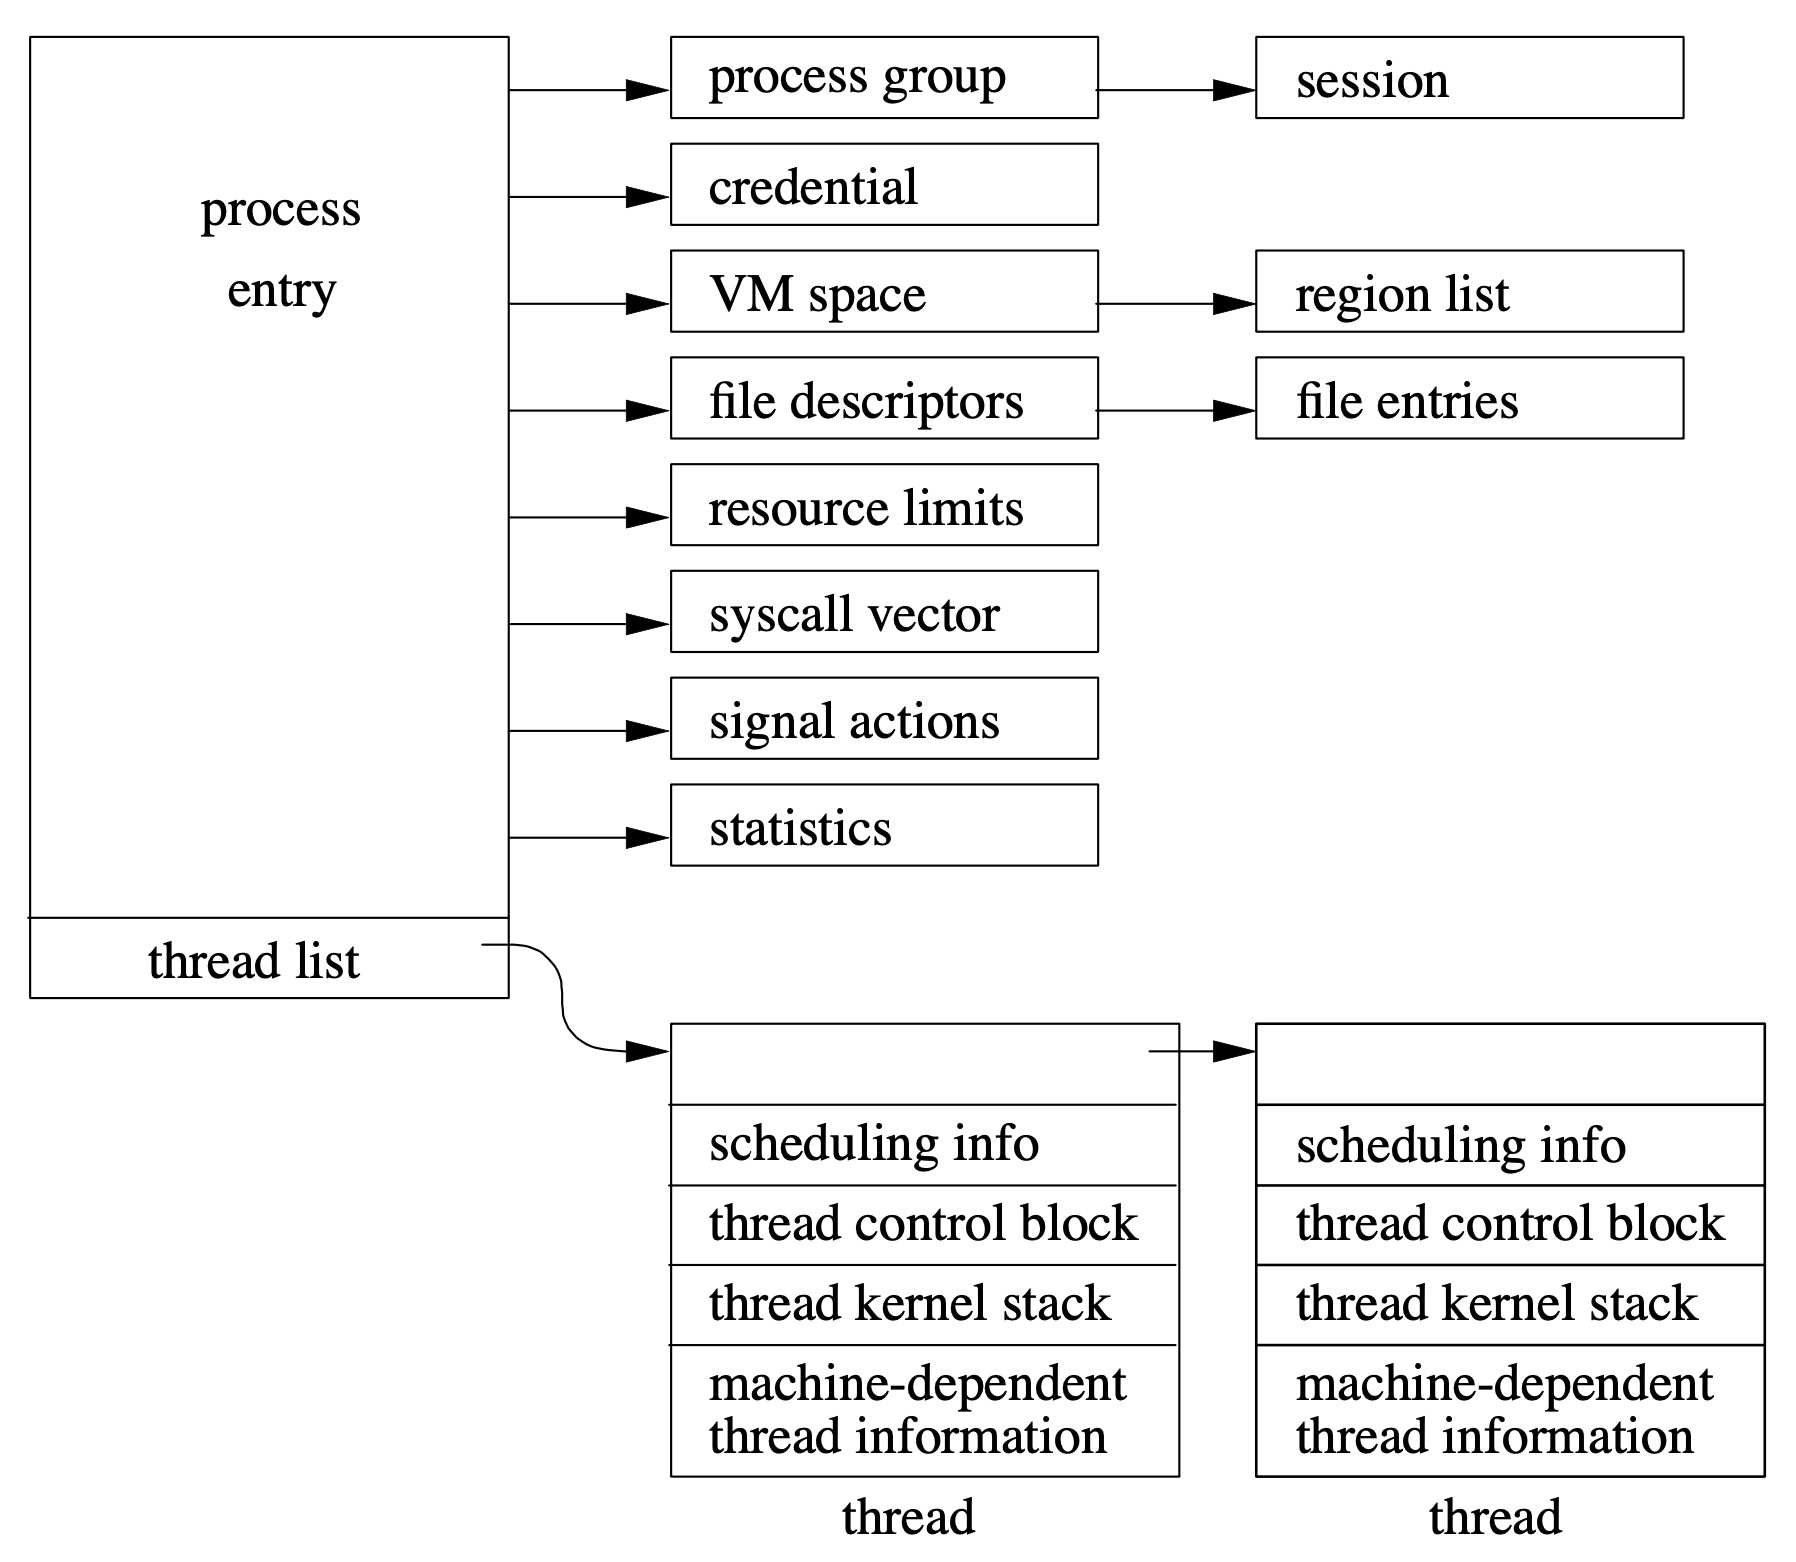
\includegraphics[width=0.5\textwidth]{images/processStructure.png}
    \caption{Estructura simplificada de un proceso.}
    \label{fig:process-state}
\end{figure}

Cada proceso cuenta con los punteros \textit{p\_pptr}, \textit{p\_children} y \textit{p\_sibling}, utilizados para establecer la relacion entre procesos. Cuando se crea un proceso hijo, se agrega a la lista \textit{p\_children} de su padre. El proceso hijo también mantiene un enlace a su padre mediante su puntero \textit{p\_pptr}. Si un proceso tiene más de un hijo activo al mismo tiempo, los hijos están asociados entre sí a través de las entradas de la lista \textit{p\_sibling}. La Figura \ref{fig:process-hierarchy} muestra un ejemplo de jerarquia de procesos.

\begin{figure}[H]
    \centering
    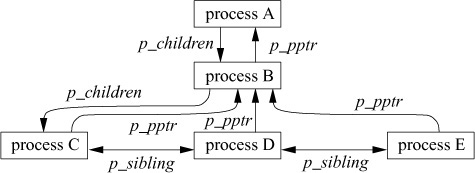
\includegraphics[width=0.5\textwidth]{images/process-hierarchy.jpeg}
    \caption{Jerarquía de grupo de procesos.}
    \label{fig:process-hierarchy}
\end{figure}


\subsubsection{Estructura de los hilos}
Un hilo, en sistemas operativos modernos, constituye una unidad fundamental de ejecución dentro de un proceso. Se trata de una entidad independiente que representa una secuencia de instrucciones ejecutables dentro del contexto de un proceso. Cada hilo posee su propio contador de programa, registros de CPU y pila de ejecución, lo que le permite ejecutar código de manera concurrente dentro del mismo proceso. Aunque los hilos comparten recursos como el espacio de direcciones y otros recursos del proceso principal, también pueden comunicarse y cooperar entre sí para llevar a cabo tareas específicas de manera más eficiente.\par

En el caso de FreeBSD, el sistema adopta el modelo 1:1, donde cada hilo de usuario se corresponde con un hilo a nivel de kernel para mejorar la eficiencia de las aplicaciones.\par

La estructura de un hilo, que se muestra en la Figura \ref{fig:process-state}, contiene la información necesaria para ejecutarse en el kernel del sistema operativo:

\begin{itemize}
    \item Información para la planificación: se refiere a la prioridad del hilo en modo kernel y en modo usuario, la cantidad de tiempo que ha pasado suspendido y el uso reciente de la CPU. Además, se indica el estado de ejecución del hilo, banderas de estado adicionales; y si el hilo se encuentra suspendido, información sobre el canal y evento por el cual espera.
    \item TSB (thread state block): estado de ejecución del hilo en modo usuario y modo kernel. La estructura incluye registros de propósito general, punteros de pila, contador de programa, registros de gestión de memoria, entre otros.
    \item Pila del kernel: pila para usar al ejecutar en el kernel. Las pilas del kernel deben mantenerse pequeñas para evitar desperdiciar memoria física.
    \item Estado de la máquina (\textit{machine-dependent state}): se refiere a la información del hilo en relación a detalles que son específicos de la arquitectura de la CPU (registros de estado de punto flotante, información de interrupciones, información de registros de segmento de memoria, etc.).
\end{itemize}

\subsubsection{Estados de los procesos e hilos}

La estructura de un proceso en FreeBSD incluye un campo que indica su estado actual. Los estados de un proceso son fundamentales para entender su comportamiento en el sistema y están estrechamente relacionados con el funcionamiento del planificador 4BSD. Cuando se crea un proceso utilizando la llamada al sistema \textit{fork}, inicialmente se marca como nuevo (NEW). Este estado indica que el proceso está en su fase de creación y aún no ha recibido suficientes recursos para comenzar la ejecución.

Una vez que se asignan los recursos necesarios, el estado del proceso se cambia a NORMAL. En este estado, los hilos del proceso pueden encontrarse en diferentes subestados: ejecutable (RUNNABLE) cuando están listos para ejecutarse o actualmente en ejecución, durmiendo (SLEEPING) cuando están esperando un evento, o detenidos (STOPPED) cuando han sido pausados por una señal o por el proceso padre. El estado NORMAL persiste hasta que el proceso completa su tarea.

Cuando un proceso ha finalizado su ejecución, entra en el estado ZOMBIE. En este estado, el proceso ha liberado sus recursos pero aún no ha notificado formalmente su terminación al proceso padre. Es responsabilidad del sistema operativo limpiar los procesos en estado ZOMBIE y comunicar al proceso padre que el hijo ha finalizado.

La relación entre estos estados y el planificador 4BSD es crucial para comprender cómo se gestionan los recursos del sistema y cómo se asigna el tiempo de CPU a los procesos en FreeBSD.

En la tabla \ref{tabla:estados-proceso}, se proporciona una descripción concisa de cada estado del proceso y su significado en el contexto del sistema operativo.

\begin{table}[H]
    \centering
    \begin{tabular}{@{}ll@{}}
    \textbf{Estado} & \textbf{Características} \ \midrule
    NEW & En fase de creación, aún sin recursos asignados \
    NORMAL & Ejecución activa, sus hilos alternaran entre \textit{RUNNABLE}, \textit{SLEEPING} o \textit{STOPPED} \
    ZOMBIE & En fase de finalización \ \bottomrule
    \end{tabular}
    \caption{Descripción de los estados del proceso en FreeBSD}
    \label{tabla:estados-proceso}
\end{table}

En FreeBSD, el sistema organiza las estructuras de procesos en dos listas principales: \textit{zombproc} y \textit{allproc}. Los procesos en estado ZOMBIE se encuentran en la lista \textit{zombproc}, mientras que los procesos activos están en la lista \textit{allproc}. Esta distinción permite optimizar las operaciones del sistema, como la llamada al sistema \textit{wait} que busca procesos terminados, así como las operaciones del planificador que identifican procesos listos para ejecutarse.

Los hilos de un proceso, por su lado, excluyendo los que están en ejecución, se distribuyen en tres colas principales: \textit{run_queue}, \textit{sleep_queue} y \textit{turnstile_queue}. Los hilos listos para ejecutarse se ubican en la \textit{run_queue}, mientras que aquellos que están bloqueados esperando eventos se encuentran en la \textit{sleep_queue} o en la \textit{turnstile_queue}. Es importante destacar que las colas \textit{run_queue} están organizadas según la prioridad de planificación de hilos establecida por el planificador 4BSD. La diferencia entre la \textit{turnstile_queue} y la \textit{sleep_queue}, radica en que esta última se utiliza para hilos bloqueados con locks de tipo \textit{sleepable}, mientras que la \textit{turnstile_queue} alberga hilos bloqueados con locks de tipo \textit{non-sleepable}.

\subsubsection{Prioridad de los hilos}

Las prioridades de los hilos son un componente importante para la planificación. Estas prioridades, que van desde 0 hasta 255 (donde 0 denota la prioridad más alta), determinarán el orden en que se ejecutarán los hilos. En la Tabla \ref{tabla:prio_hilos}, se describen los diferentes rangos de prioridades.

Las prioridades en el rango de 0 a 47 son asignadas de forma predeterminada por el sistema y se destinan a las tareas de interrupción.\par

Las prioridades de los hilos en tiempo real se encuentran en el intervalo de 48 a 79 y deben ser configuradas previamente por las aplicaciones mediante la llamada al sistema \textit{rtprio}. A continuación, se encuentran los hilos con prioridades en el rango de 80 a 119, conocidos como hilos del kernel superior (top-half kernel threads). Estos hilos se encargan de gestionar operaciones críticas del kernel que afectan a todo el sistema.\par

Los hilos con prioridades entre 120 y 223 pertenecen a la clase de hilos de tiempo compartido. Están destinados a ejecutar tareas de usuario convencionales y sus prioridades son ajustadas de manera automática por el kernel en función del uso de la CPU.\par

Cuando no hay tareas activas que requieran el uso de la CPU, los hilos de la clase "IDLE" pueden ejecutarse. Estos hilos tienen la finalidad de mantener el sistema en un estado inactivo, consumiendo recursos mínimos y estando listos para responder a tareas prioritarias.\par

\begin{table}[H]
    \centering
    \begin{tabular}{|c|c|c|}
        \hline
        \textbf{Rango} & \textbf{Clase} & \textbf{Tipo de hilo} \\
        \hline
        0 - 47 & ITHD & Bottom-half kernel (interrupt) \\
        \hline
        48 -79 & REALTIME & Real-time user \\
        \hline
        80 - 119 & KERN & Top-half kernel \\
        \hline
        120 - 223 & TIMESHARE & Time-sharing user \\
        \hline
        224 - 255 & IDLE & Idle user \\
        \hline
    \end{tabular}
    \caption{Clases de hilos por rango de prioridad.}
    \label{tabla:prio_hilos}
\end{table}


\subsection{Planificación}

Planificar es decidir cómo, cuándo y por cuánto tiempo vamos a correr los hilos que se encuentran en nuestro sistema; tanto los hilos propios del sistema operativo, como de aplicaciones que se encuentran en ejecución.\par

En este sentido, la planificación es fundamental para equilibrar la utilización de los recursos con el tiempo necesario para completar los programas. FreeBSD implementa por defecto, un planificador \textit{compartido por tiempo}, el cual calcula la prioridad de los procesos de manera periódica. Este cálculo se realiza en base a datos previos, como la cantidad de tiempo utilizado de CPU o la cantidad de recursos de memoria que el proceso mantiene o requiere para su ejecución. No obstante, algunas tareas requieren un control más preciso sobre el proceso, como el caso de la planificación de tiempo real. FreeBSD también implementa esta funcionalidad mediante una cola separada para los hilos en cuestión, los cuales no se ven interrumpidos por otros hilos a menos que tengan igual o mayor prioridad.\par

Además, el \textit{kernel} de FreeBSD cuenta con una cola de hilos de mínima prioridad que se ejecutan únicamente cuando ningún otro hilo en las colas de mayor prioridad está en un estado de posible ejecución.\par

En cuanto al método de planificación por tiempo, FreeBSD favorece a los programas interactivos. Asigna una prioridad alta a cada hilo y permite que se ejecute por un periodo fijo de tiempo, conocido como \textit{time slice}. A medida que el hilo se ejecuta, su prioridad disminuye, mientras que aquellos suspendidos por E/S mantienen su prioridad. Por su parte, los hilos que se mantienen inactivos mejoran su prioridad en la cola.\par

TIENE QUE SER MAS LARGA. VER COMO ALARGAR.

\subsection{Conceptos del proyecto integrador previo}

% El scheduler se encarga de planificar aquellos hilos correspondientes a procesos en estado NORMAL. Los hilos que conforman un proceso pueden encontrarse en diferentes estados:

% \begin{itemize}
%     \item \uppercase{inactive}: En proceso de creación y aún no han sido inicializados.
%     \item \uppercase{inhibited}: Esperando por algún recurso del sistema o evento antes de poder ejecutarse.
%     \item \uppercase{can\_run}: Inicializados y disponibles para ser agregados a alguna cola de ejecución.
%     \item \uppercase{runq}: En la cola de ejecución, esperando su turno para ser ejecutados.
%     \item \uppercase{running}: En ejecución.
% \end{itemize}

\subsubsection{Introducción}

El proyecto integrador del cual partimos, consiste en modelar el planificador 4BSD con Redes de Petri. Los hilos de ejecución de un proceso como el planificador del sistema operativo pueden considerarse como sistemas que pueden modelarse utilizando esta herramienta.\par

Las decisiones de encolado de los hilos en una CPU se toman a partir de la información representada en el modelo; así como también los estados globales y los de cada hilo.\par

\textcolor{red}{agregar alguito pa no pasar tan duracell}

\subsubsection{Elección del planificador}

La planificación a corto plazo en FreeBSD ha experimentado una notable evolución a lo largo de los años. Desde sus inicios con el planificador 4BSD hasta el actual planificador ULE, se han implementado cambios significativos que han contribuido a mejorar la eficiencia y el rendimiento del sistema.\par

Aunque el planificador ULE es el predeterminado en las versiones actuales de FreeBSD, este trabajo se basa en el trabajo previo realizado en el marco del proyecto integrador, que se centró en el planificador 4BSD\@. Para entender con mayor detalle y contexto dicha elección, visitar la sección 2.3.3.\ del proyecto integrador previo\cite{bib1}.

En este momento, nuestro enfoque principal no radica en realizar un cambio inmediato en el sistema operativo ni en contribuir directamente a la comunidad de FreeBSD\@. En su lugar, estamos continuando con la fase de investigación e implementación centrada en este tipo de planificadores.\par

Al mismo tiempo, el planificador 4BSD ha sido mantenido por la comunidad de FreeBSD durante décadas y no hay planes inmediatos para dejar de darle soporte. Esto significa que todavía sigue siendo una opción estable y confiable para el desarrollo de nuestro proyecto.\par


--- PLANIFICADOR

\subsubsection{Funcionamiento del planificador 4BSD}

El planificador 4BSD, inicialmente diseñado para sistemas monoprocesador, ha evolucionado para adaptarse eficazmente a sistemas multiprocesador. Comprender su funcionamiento es esencial para apreciar cómo este componente crítico del sistema FreeBSD gestiona la asignación de recursos y el tiempo de ejecución de los hilos.\par

En esencia, el planificador 4BSD organiza los hilos en múltiples colas según su prioridad. Cada hilo tiene una prioridad asignada y reside en una cola específica de acuerdo con esta prioridad.\par

Un aspecto crucial del planificador 4BSD es la gestión de tiempos de ejecución equitativos. A cada proceso se le asigna un pequeño período de tiempo, conocido como "timeslice". Una vez que un proceso agota su timeslice, se suspende temporalmente para permitir que otros procesos tengan la oportunidad de ejecutarse. Este proceso cíclico de asignación de tiempos de ejecución, basado en el algoritmo "Round Robin", asegura que ningún proceso monopolice los recursos del sistema durante largos períodos, contribuyendo así a un rendimiento estable y justo del sistema,  garantizando la equidad en el uso de los recursos del sistema.\par

En lo que respecta a las prioridades, el planificador 4BSD las ajusta periódicamente en función del tiempo de CPU consumido por cada hilo. Este proceso implica elevar la prioridad de los hilos que han utilizado menos tiempo de CPU y reducir la prioridad de aquellos que han consumido más recursos de procesador. De esta manera, el planificador se encarga de equilibrar la carga de trabajo de manera equitativa entre todos los procesos en ejecución en el sistema.\par


\subsubsection*{Funciones basicas del planificador}

intro en donde se explica que todas las funciones de aca abajo basicamente fueron las que tuvieron que cambiar para la planificacion con RdP

\textcolor{red}{Encolado (add)}
El sistema usa 64 colas, seleccionando una cola para un determinado hilo y dividiendo la prioridad del hilo por 4. Para ahorrar tiempo, los hilos en cada cola no se vuelven a dividir en prioridades.\par

Estas colas pueden ser de tipo run queue, turnstile queue o sleep queue. Los hilos en estado RUNNABLE se ubican en las colas de tipo run queue; mientras que los que están bloqueados o esperando un evento, son posicionados en los otros dos tipos de colas.\par

Si un hilo agota su tiempo (o intervalo de tiempo) permitido, se coloca al final de la cola de la que procede, y el próximo hilo (ahora al principio de la cola) se selecciona para ejecutarse.\par

Si un hilo se bloquea, no se vuelve a colocar en la cola de ejecución (run queue). En su lugar, se coloca en una turnstile queue o en una sleep queue.\par

Las operaciones relacionadas al encolado se realizan dentro de la función sched\_add(). Ésta función recibe como parámetros el hilo a encolar y flags con información acerca del mismo.\par

Su primera tarea es corroborar que el hilo se encuentre en un estado permitido para ser encolado, es decir, en estado CAN\_RUN o RUNNING. Al pasar esta verificación, se adquiere el lock del planificador y se lo pasa al estado RUNQ para luego elegir en cuál cola de CPU va a ser asignado. Esto es posible a través de la función sched\_pickcpu(), la cual elige un CPU de la siguiente forma:

\begin{enumerate}
    \item Consulta si el hilo ya se había ejecutado en un procesador anterior y si es posible volverlo a encolar en el mismo. En caso de que sea verdadero, almacena este valor en una variable. En caso contrario, dentro de esa variable guarda el valor NOCPU (igual a -1).
    \item Luego itera a través de cada CPU disponible en el sistema. En caso de que el CPU que se está iterando no permita el encolado, continúa con el siguiente.
    \item Para el caso en que esté permitido el encolado para el CPU que se está iterando, existen dos opciones basadas en el valor de la variable inicializada en el primer punto.
    \begin{enumerate}
        \item En caso de que la variable haya sido inicializada con el valor NOCPU, se la sobreescribe con el CPU de la iteración en la que se encuentra el programa en ese momento.
        \item En caso de que la variable haya sido inicializada con el valor del último CPU en el que había sido ejecutado el hilo, se consulta si la cola del CPU que se está iterando, tiene menor cantidad de procesos que la del CPU elegido en el punto 1. Caso afirmativo, se reemplaza el valor de la variable por el CPU que se está iterando, ya que esto significa que éste procesador contiene menos hilos en su cola de ejecución. Caso contrario, el valor de la variable no se sobreescribe.
    \end{enumerate}
    \item Al finalizar la iteración de cada CPU, se retorna el valor de la variable con el CPU más apropiado para el hilo.
\end{enumerate}

Una vez elegido el mejor CPU para el hilo, se procede a realizar los cambios de contexto necesarios para agregarlo a la cola del procesador correspondiente.

Si el procesador al que se agrega el hilo es diferente al que está ejecutando la función en ese instante, éste último envía una señal IPI (inter-processor interrupt) para comunicar que existe este nuevo hilo en su cola.

En caso de que el hilo se agregara a la cola del CPU actual, se llama a las funciones correspondientes para saber si este hilo tiene mayor prioridad que el que está en ejecución actualmente y debe reemplazarlo, esto se conoce como preemption.

\textcolor{red}{Cambios de contexto (switch y throw)}
Al hablar de cambios de contexto de los hilos, se hace referencia a dos funciones en particular.\par

La función sched\_switch() se encarga de expulsar al hilo que recibe por parámetro (hilo actual en ejecución), o en caso de que el hilo continúe en estado RUNNING por alguna razón, se vuelve a poner en cola a través de la función sched\_add().\par

Una vez finalizada la expulsión se solicita un nuevo hilo para ejecutar. Esto se hace a través de la función choosethread() y sched\_choose().\par

Una vez obtenido el nuevo hilo, se verifica que éste no sea el mismo que fue puesto en cola anteriormente, si esto sucediera, sólo continúa la ejecución. Pero en caso de que sean dos hilos diferentes, se procede a realizar el cambio de contexto haciendo uso de la función cpu\_switch().\par

La función cpu\_switch() guarda el contexto del hilo anterior y restaura el contexto del nuevo hilo. Así como también, se asegura de que el estado del nuevo hilo se marque como TD\_RUNNING (en ejecución).\par

Otra de las funciones que se encargan del cambio de contexto es sched\_throw(), la cual se encarga de cambiar un hilo por otro en el mismo CPU que se está ejecutando. Recibe un hilo como parámetro (el cual puede ser nulo), y lo expulsa del planificador. Luego a través de la misma función utilizada anteriormente, choosethread(), obtiene un nuevo hilo y continúa con su ejecución.\par

\textcolor{red}{Elección de hilos (choose)}
La elección del próximo hilo a ejecutar se hace a través de la función sched\_choose() previamente invocada por la función choosethread() nombrada anteriormente.

El funcionamiento consiste en elegir al hilo con mayor prioridad dentro de alguna de las colas no vacías del CPU o de la cola global. Cada hilo habilitado para ser ejecutado, es decir en estado RUNNABLE, tiene una prioridad asignada.

La función comienza obteniendo el primer hilo de la cola global y el primero de la cola del CPU; guardando ambos en dos variables diferentes. Luego compara las prioridades de ambos y se queda con el de mayor prioridad.

Una vez elegido el hilo, se procede a removerlo de la cola correspondiente, ya sea la global o la del CPU, y se retorna este hilo.

Para el caso en que ambos hilos sean nulos, es decir, no hay hilos para ejecutar, se simula una ejecución con el idlethread y se retorna el mismo.

\textcolor{red}{Remoción de hilos de la cola (rem)}
A diferencia de la función anterior, en la que al elegir un hilo para correr, éste era removido de la cola en la que estaba ubicado, la función sched\_rem() se utiliza para quitar un hilo (especificado por parámetro) de una cola por dos razones principales.\par

Una de estas es el ajuste de prioridad que consiste en otorgarle una nueva prioridad al hilo por lo que es necesario removerlo de la cola en la que se encuentra y luego volver a encolarlo a través de la función sched\_add() en la posición correspondiente.\par

El otro motivo por el cual se querría hacer uso de esta función es en caso de que un hilo tenga afinidad con algún CPU, por lo que el procedimiento será igual al mencionado en el párrafo anterior, con el objetivo de que se encuentre en la cola correcta.\par


----- RED DE PETRI

\subsubsection{Modelado del hilo}
Uno de los modelos representados a través de la Red de Petri, es el de los estados de un hilo. En la figura es posible observar esta representación.\par

\textcolor{red}{Agregar red de petri del hilo}

\begin{itemize}
    \item \textbf{T0\_INIT}: El paso del estado INACTIVE a CAN\_RUN. Esto sucede cuando el hilo se agrega al planificador. Esto sucede generalmente en el momento de creación de un proceso o cuando el mismo realiza un fork. Esta tarea no corresponde al scheduler, por lo que inicialmente un hilo en el planificador se encuentra inicializado en el estado CAN\_RUN. Esta transición nunca se dispara, solo se la incorpora al modelo de modo representativo.
    \item \textbf{T1\_ON\_QUEUE}: El hilo se pone en una cola local de una determinada CPU o en la cola global dependiendo de la disponibilidad. Esta cola organiza los hilos de acuerdo a sus prioridades de ejecución.
    \item \textbf{T2\_SET\_RUNNING}: El hilo se quita de la cola y pasa a ejecutar las instrucciones del programa que tiene asignadas. En este instante el procesador se encuentra ocupado por dicho hilo.
    \item \textbf{T3\_SWITCH\_OUT}: El scheduler interrumpe el hilo y lo vuelve a colocar en una cola. El planificador toma otro hilo de la cola (el de mayor prioridad) y realiza un cambio de contexto.
    \item \textbf{T4\_TO\_WAIT\_CHANNEL}: Algún evento, semáforo o espera bloquea al hilo. Se agrega en una sleep queue o turnstile, en la cual el hilo queda a la espera de un evento que le quitará el bloqueo.
    \item \textbf{T5\_WAKEUP}: Se desbloquea el hilo y puede volver a encolarse nuevamente. El evento que lo desbloquea se genera fuera del scheduler. El hilo queda a la espera para poder cambiar de estado cuando corresponda.
    \item \textbf{T6\_REMOVE}: Se ejecutará cada vez que un hilo deba ser expulsado de la cola en que se encuentra actualmente.
\end{itemize}


\subsubsection{Modelado del planificador}

Para modelar el planificador se hace un modelo específico para un procesador y se extiende para los demás. En este proyecto se consideran cuatro procesadores.

\textcolor{red}{Agregar red de petri de 1 procesador}

Transiciones
\begin{itemize}
    \item TRAN\_ADDTOQUEUE: Un hilo es agregado a la cola del CPU correspondiente. Se encuentra inhibida cuando todo el sistema se encuentra en modo monoprocesador (al inicio del sistema operativo); y cuando ya existe un hilo en la cola.
    \item TRAN\_UNQUEUE: Se quita al hilo próximo a ejecutar de la cola del CPU. En este punto el hilo se encuentra listo para ser ejecutado.
    \item TRAN\_EXEC: El hilo pasa a ejecución por lo que el recurso del procesador se encuentra ocupado. Esta transición elimina el token de la plaza de habilitación, permitiendo así que un nuevo hilo pueda ser encolado. A su vez, ésta transición se encuentra inhibida en el modo monoprocesador.
    \item TRAN\_EXEC\_EMPTY: Esta transición se comporta de igual manera que la anterior, pero no depende de la plaza de habilitación. Su utilidad surge para los hilos provenientes de la cola global.
    \item TRAN\_RETURN\_VOL: Representa un retorno del recurso procesador para que pueda ejecutar otro hilo de su cola. Más precisamente, se dispara cuando la interrupción de la ejecución se debe a que el hilo no puede continuar porque espera por un evento o un recurso.
    \item TRAN\_RETURN\_INVOL: El funcionamiento es igual a la transición anterior, pero en este caso se dispara cuando la interrupción se produce porque el hilo consumió su tiempo asignado de CPU o bien finalizó su tarea.
    \item TRAN\_FROM\_GLOBAL\_CPU: Representa el desencolado de un hilo desde la cola global.
    \item TRAN\_REMOVE\_QUEUE: Expulsa un hilo de la cola y también resta un token de habilitación de la CPU, es decir, se premia a la misma para que pueda encolar.
    \item TRAN\_REMOVE\_EMPTY\_QUEUE: Su funcionamiento es igual al anterior pero se ejecuta en los casos en que la plaza de habilitación no posea ningún token.
    \item TRAN\_REMOVE\_GLOBAL\_QUEUE: Expulsa un hilo de la cola global. No premia al CPU.
    \item TRAN\_START\_SMP: Se dispara cuando el sistema pasa de monoprocesador a multiprocesador.
    \item TRAN\_THROW: Se ejecutará automáticamente cada vez que todas las plazas de habilitación de las CPU tengan al menos un token. El objetivo de esta transición consiste en habilitar las colas con la menor cantidad de hilos que estaban inhibidas, una vez que todas se han emparejado.
    \item TRAN\_QUEUE\_GLOBAL: Agrega un hilo a la cola global.
\end{itemize}


\subsubsection{Jerarquía de transiciones}
Para llevar a cabo la conexión entre las redes de los hilos y la red de recursos de las CPU se utiliza el concepto de redes jerárquicas. Es decir que al dispararse cierta transición en la red de recursos, también debe dispararse su transición correspondiente en la red del hilo.

Las jerarquías están definidas de la siguiente forma:
\begin{itemize}
    \item Transiciones TRAN\_ADDTOQUEUE y TRAN\_QUEUE\_GLOBAL de la red de recursos son jerárquicas a la transición T1\_ON\_QUEUE del hilo.
    \item Transiciones TRAN\_EXEC y TRAN\_EXEC\_EMPTY de la red de recursos son jerárquicas a la transición T2\_SET\_RUNNING del hilo.
    \item Transiciones TRAN\_REMOVE\_QUEUE, TRAN\_REMOVE\_EMPTY\_QUEUE y TRAN\_ REMOVE\_GLOBAL\_QUEUE de la red de recursos son jerárquicas a la transición T6\_ REMOVE del hilo.
    \item Transición TRAN\_RETURN\_INVOL de la red de recursos es jerárquica a la transición T3\_ SWITCH\_OUT del hilo.
    \item Transición TRAN\_RETURN\_VOL de la red de recursos es jerárquica a la transición T4\_TO \_WAIT\_CHANNEL del hilo.
\end{itemize}

\subsubsection{Marcado inicial}
La red de recursos se inicializará siempre con un token en la plaza que indica que el sistema se encuentra funcionando en modo monoprocesador. Además, se inicializan las plazas que representan a las CPU con un token, excepto la de la CPU0 ya que la misma, inicialmente se encuentra ejecutando el hilo inicial del sistema, por lo que esta última debe inicializarse con un token en la plaza de ejecución (PLACE\_EXECUTING\_0).



\section{Desarrollo}

\subsection{Introducción}
En el marco de este trabajo de investigación, implementamos mejoras en el planificador a corto plazo basado en Redes de Petri para el sistema operativo FreeBSD. Este proyecto supuso un gran desafío, ya que implicó comprender y depurar el código previo y los archivos del código fuente de FreeBSD relacionados con el funcionamiento del scheduler 4BSD, que había sido desarrollado por estudiantes de nuestra misma institución en un proyecto integrador previo. Fue un proceso arduo de lectura y relectura constante, con el objetivo de adquirir un panorama general y detallado sobre el funcionamiento del scheduler.\par

\subsection{Metodologías de trabajo}
Luego de superar la fase inicial, dedicamos un tiempo a planificar la forma en que íbamos a abordar el desarrollo del proyecto. Creíamos crucial establecer una estructura organizada para avanzar de manera sistemática y dejar registros detallados de nuestras actividades en cada etapa del proyecto, lo cual podría ser útil para trabajos futuros.\par
Durante esta fase, nos enfocamos en documentar los procesos de instalación y depuración, establecer una estrategia de ramas estandarizada en el repositorio fork de FreeBSD y definir un repositorio externo donde alojar todos los recursos que podrían ser útiles para cualquier persona que desee involucrarse en la implementación del proyecto. Estas tareas fueron de gran importancia para asegurarnos de que estábamos trabajando de manera ordenada y eficiente, y para crear un recurso valioso para la comunidad.\par

\subsubsection{Estrategia de ramificación}
Definir una estrategia de ramificación o branch strategy en los proyectos es importante porque ayuda a mantener el control sobre el flujo de trabajo, a mantener la organización del proyecto y a asegurar que las modificaciones se integren sin problemas en la rama principal del código. Una estrategia de ramificación bien definida establece un conjunto de reglas claras y consistentes para crear y fusionar ramas de código.\par

Al mismo tiempo, ayuda a mantener un historial completo y bien organizado de las modificaciones realizadas al código, lo que puede ser útil para fines de seguimiento y continuidad del proyecto. Por esta razón, definimos el prefijo de branches conformado por los apellidos de los integrantes del grupo de trabajo, en nuestro caso, por ejemplo, DrudiGoldmanPI/. Esto también nos ayuda a encontrar con mayor facilidad todos los cambios realizados en este proyecto integrador.\par

\textcolor{red}{Mostrar las branch strategies}

\subsubsection{Conventional commits}
Los Conventional Commits son una herramienta esencial para mantener una estructura y formato consistente en los mensajes de confirmación del código. En el contexto de un trabajo de tesis, su importancia radica en que el trabajo probablemente seguirá avanzando con el tiempo por otros alumnos o personas que deseen seguir el mismo camino.\par

El uso de Conventional Commits ayuda a mantener una estructura bien organizada de los pequeños pasos que se fueron dando en cada una de las ramas, lo que permite a cualquier persona que consulte el repositorio tener una comprensión clara y rápida del progreso del proyecto y de los cambios que se realizaron en cada paso.\par

\subsubsection{Pruebas del kernel}
La depuración del kernel es una tarea crucial en el desarrollo de sistemas operativos, ya que permite encontrar y corregir errores que de otra manera podrían pasar desapercibidos. En nuestro trabajo, la herramienta protagonista en este ámbito, fue KGDB.\par

kgdb permite la depuración de archivos de núcleo del kernel. Cuando se produce un kernel panic o una falla del sistema, podemos utilizar esta herramienta para analizar el dump core y encontrar la causa subyacente del problema. Dentro de  este modo, podemos examinar el estado del sistema en el momento de la falla y determinar qué parte del código del kernel causó la falla.\par







\section{Análisis de resultados integrales}
\label{ch:results}

En este capítulo, se presentan los resultados integrales de nuestra investigación, que se centra en dos aspectos cruciales para la optimización de la gestión de recursos en sistemas operativos. En primer lugar, introduciremos los resultados del módulo de Encendido y Apagado de Procesadores. En segundo lugar, se presentarán los del módulo de Monopolización de Núcleos.\par

Ambos mecanismos desarrollados proporcionan al sistema operativo y a la red las herramientas necesarias para mejorar la gestión de sus recursos. Es fundamental tener presente que estos mecanismos representan un paso esencial hacia la consecución de objetivos más amplios, específicamente relacionados con mejoras en la eficiencia energética y el rendimiento general del sistema. La exposición de resultados tiene como objetivo destacar la funcionalidad adecuada de la implementación de los módulos previamente desarrollados en este informe, acercándonos a  los objetivos más amplios mencionados.\par

Como se detalló en la sección de desarrollo de este informe, previo a  la implementación de los módulos mencionados llevamos a cabo una actualización del código del kernel, para incorporar al último lanzamiento estable de FreeBSD, las modificaciones realizadas en el proyecto integrador previo. Decidimos incluir los resultados de esta actualización al final de este capítulo, dado que consideramos que los módulos son más propensos a un análisis detallado y a comprender sus resultados. En contraste, las actualizaciones simplemente requieren que el sistema continúe funcionando correctamente.\par

\subsection{Resultados de la Implementación del Módulo de Encendido/Apagado de Procesadores}
La implementación del módulo de encendido/apagado de procesadores en FreeBSD, utilizando el enfoque de Redes de Petri, se realizó como punto de inicio del camino hacia la mejora de eficiencia y gestión de recursos del sistema operativo. En esta sección, presentaremos los resultados obtenidos de nuestras pruebas y analizaremos cómo este módulo afecta el rendimiento del sistema.\par


\subsubsection{Estado Inactivo del Sistema}
En situaciones de inactividad del sistema operativo, caracterizadas por la ausencia de tareas pendientes, cada procesador opera en un modo especial ejecutando hilos de la clase IDLE. Este escenario está diseñado para que el sistema mantenga un estado pasivo, preparado para abordar de manera eficiente cualquier tarea que pueda emerger.\par

Creemos importante resaltar que, independientemente de si nuestro módulo de encendido/apagado está activo para alguno de los procesadores en este contexto, hemos considerado y abordado esta situación en nuestra implementación para garantizar la estabilidad del sistema. La Figura \ref{fig:cpuOnOff-result-idle} proporciona una representación visual de este estado.\par

\begin{figure}[H]
    \centering
    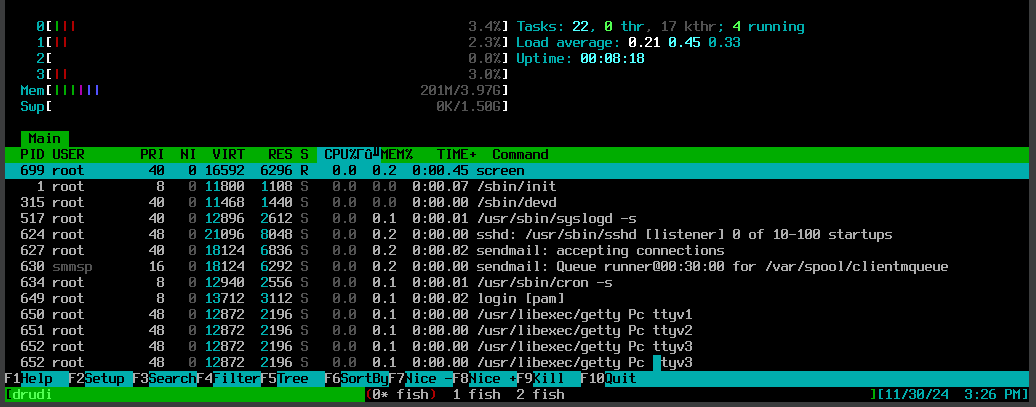
\includegraphics[width=0.8\textwidth]{images/cpuOnOff-result-idle.png}
    \caption{Estado inactivo del sistema.}
    \label{fig:cpuOnOff-result-idle}
\end{figure}

\subsubsection{Comportamiento con el Módulo Inhabilitado}
Cuando el módulo de encendido/apagado de procesadores no está habilitado para ningún núcleo, el sistema operativo sigue su funcionamiento convencional bajo la lógica del planificador. En este estado, el \textit{scheduler} opera mediante el uso de la Red de Petri  con las plazas y transiciones de cada uno de los procesadores del sistema, sin hacer uso de la adición de plazas y transiciones que corresponden al módulo, introducidas en el desarrollo del mismo.\par

Para confirmar dicho comportamiento, llevamos a cabo una prueba de estrés sobre los procesadores, ejecutando un programa que genera múltiples procesos que realizan cálculos matemáticos complejos. Durante la ejecución del programa, supervisamos el sistema y observamos que todos los procesadores operaban al máximo de su capacidad, funcionando al 100\% para completar la tarea. La Figura \ref{fig:cpuOnOff-result-full-load} proporciona una representación visual de este estado.\par

Este escenario de funcionamiento con el módulo deshabilitado proporciona un punto de referencia inicial para comprender el impacto de nuestra implementación en la gestión de recursos y el rendimiento general del sistema operativo.\par

\begin{figure}[H]
    \centering
    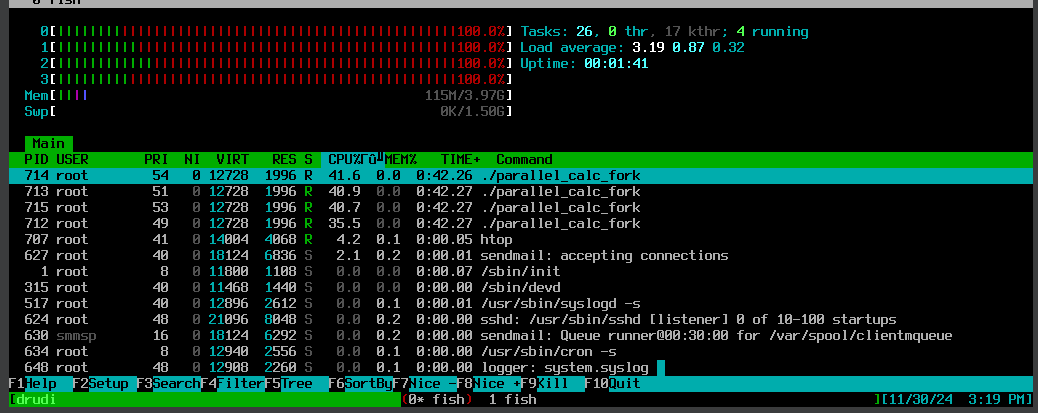
\includegraphics[width=0.8\textwidth]{images/cpuOnOff-result-full-load.png}
    \caption{Estado de los núcleos con el modulo encendido/apagado inhabilitado.}
    \label{fig:cpuOnOff-result-full-load}
\end{figure}

\subsubsection{Comportamiento con el Módulo Habilitado}
Basándonos en las observaciones anteriores, llevamos a cabo la misma prueba de estrés, pero activando previamente el módulo de encendido/apagado para inhabilitar el Procesador 2.\par

Este enfoque nos permitió no solo corroborar la funcionalidad adecuada de la implementación, sino también analizar la respuesta del sistema ante un cambio tan significativo como el bloqueo del encolado en uno de sus núcleos.\par

En relación a los resultados obtenidos durante esta evaluación, observamos que, al suspender uno de los procesadores del sistema, este continuó funcionando de manera estable. Se puede apreciar que la carga del procesador suspendido se mantuvo en cero, mientras que los demás procesadores continuaron ejecutando los cálculos. Esto demuestra de manera concluyente que el sistema fue capaz de adaptarse sin dificultades a la reducción de recursos de procesamiento.\par

\begin{figure}[H]
    \centering
    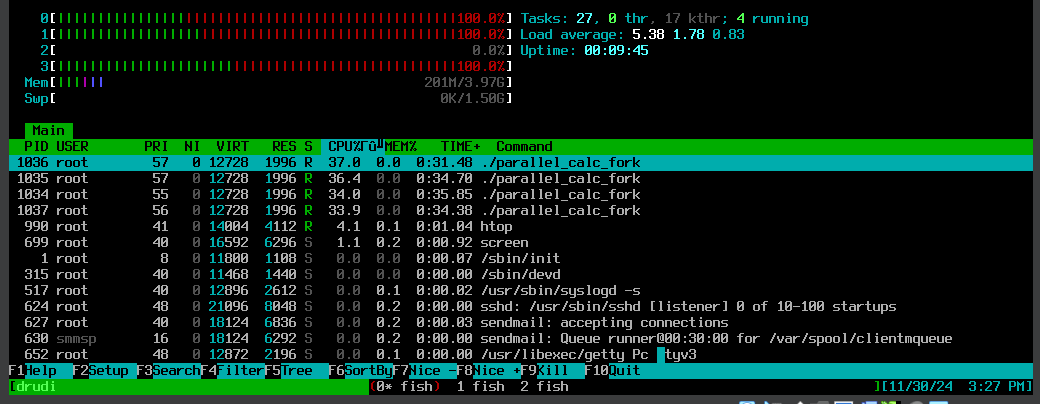
\includegraphics[width=0.8\textwidth]{images/cpuOnOff-result-1CPU.png}
    \caption{Estado de los núcleos con el modulo encendido/apagado habilitado para la CPU2.}
    \label{fig:cpuOnOff-result-1cpu}
\end{figure}

En relación al tiempo necesario para completar el cálculo del programa, notamos que dicho tiempo aumentó proporcionalmente a la disminución en el número de procesadores activos, destacando la correlación entre la disponibilidad de recursos de procesamiento y el tiempo total requerido para finalizar el programa. En la Figura \ref{fig:cpuOnOff-result-2cpu} podemos comprobar el funcionamiento del sistema con la inhabilitación simultánea de dos procesadores.\par

\begin{figure}[H]
    \centering
    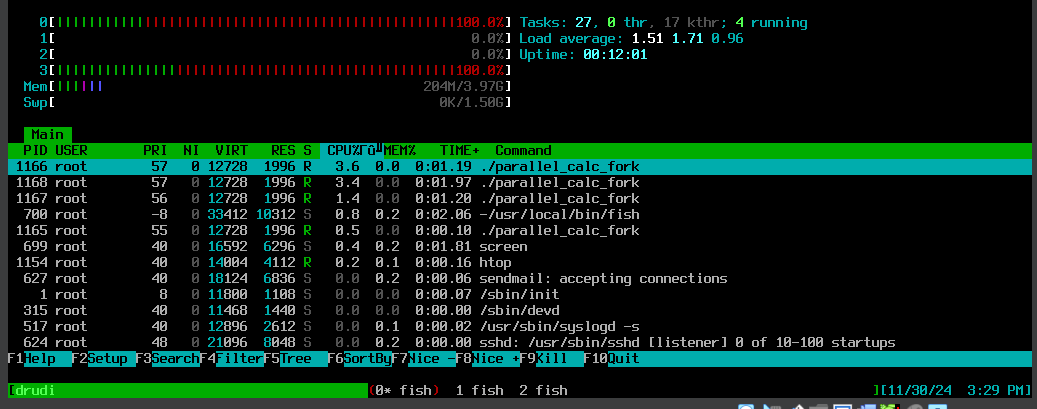
\includegraphics[width=0.8\textwidth]{images/cpuOnOff-result-2CPU.png}
    \caption{Estado de los núcleos con el modulo encendido/apagado habilitado para multiples CPUs.}
    \label{fig:cpuOnOff-result-2cpu}
\end{figure}

% TODO{TABLA CON LOS TIEMPOS DE EJECUCION CON TODOS LOS PROC, CON 3 Y CON 2 + explicacion + diciendo que el objetivo no es tener apagos los procesadores en tiempos de estres, sino que se muestra solo para ejemplificar, y que la parte del kernel que en un futuro haga uso del modulo para reducir los gastos energeticos, tiene que entender cuando conviene apagar. (Medio como conclusion del modulo)}

% TODO{branch con el codigo}


\subsection{Resultados del módulo de Monopolización de Núcleos}

La implementación del módulo de Monopolización de Núcleos en FreeBSD constituyó el próximo paso en el desarrollo de este proyecto integrador. A continuación, se expondrán en detalle los resultados alcanzados al concluir dicho módulo.\par

\subsubsection{Estado Normal del Sistema}

En este apartado se analizará el comportamiento general del sistema con el módulo de monopolización deshabilitado. Es relevante señalar que bajo esta configuración, los procesadores operan de forma predeterminada, utilizando la Red de Petri como planificador para mantener el equilibrio de la carga. De esta forma, los núcleos que en algún momento carezcan de tareas tomarán hilos de la cola global o ejecutaran hilos de clase IDLE en caso de inactividad del sistema. Con el planificador funcionando normalmente, los subprocesos se distribuyen entre los núcleos disponibles, utilizando las políticas definidas por el mismo.\par

\begin{figure}[H]
    \centering
    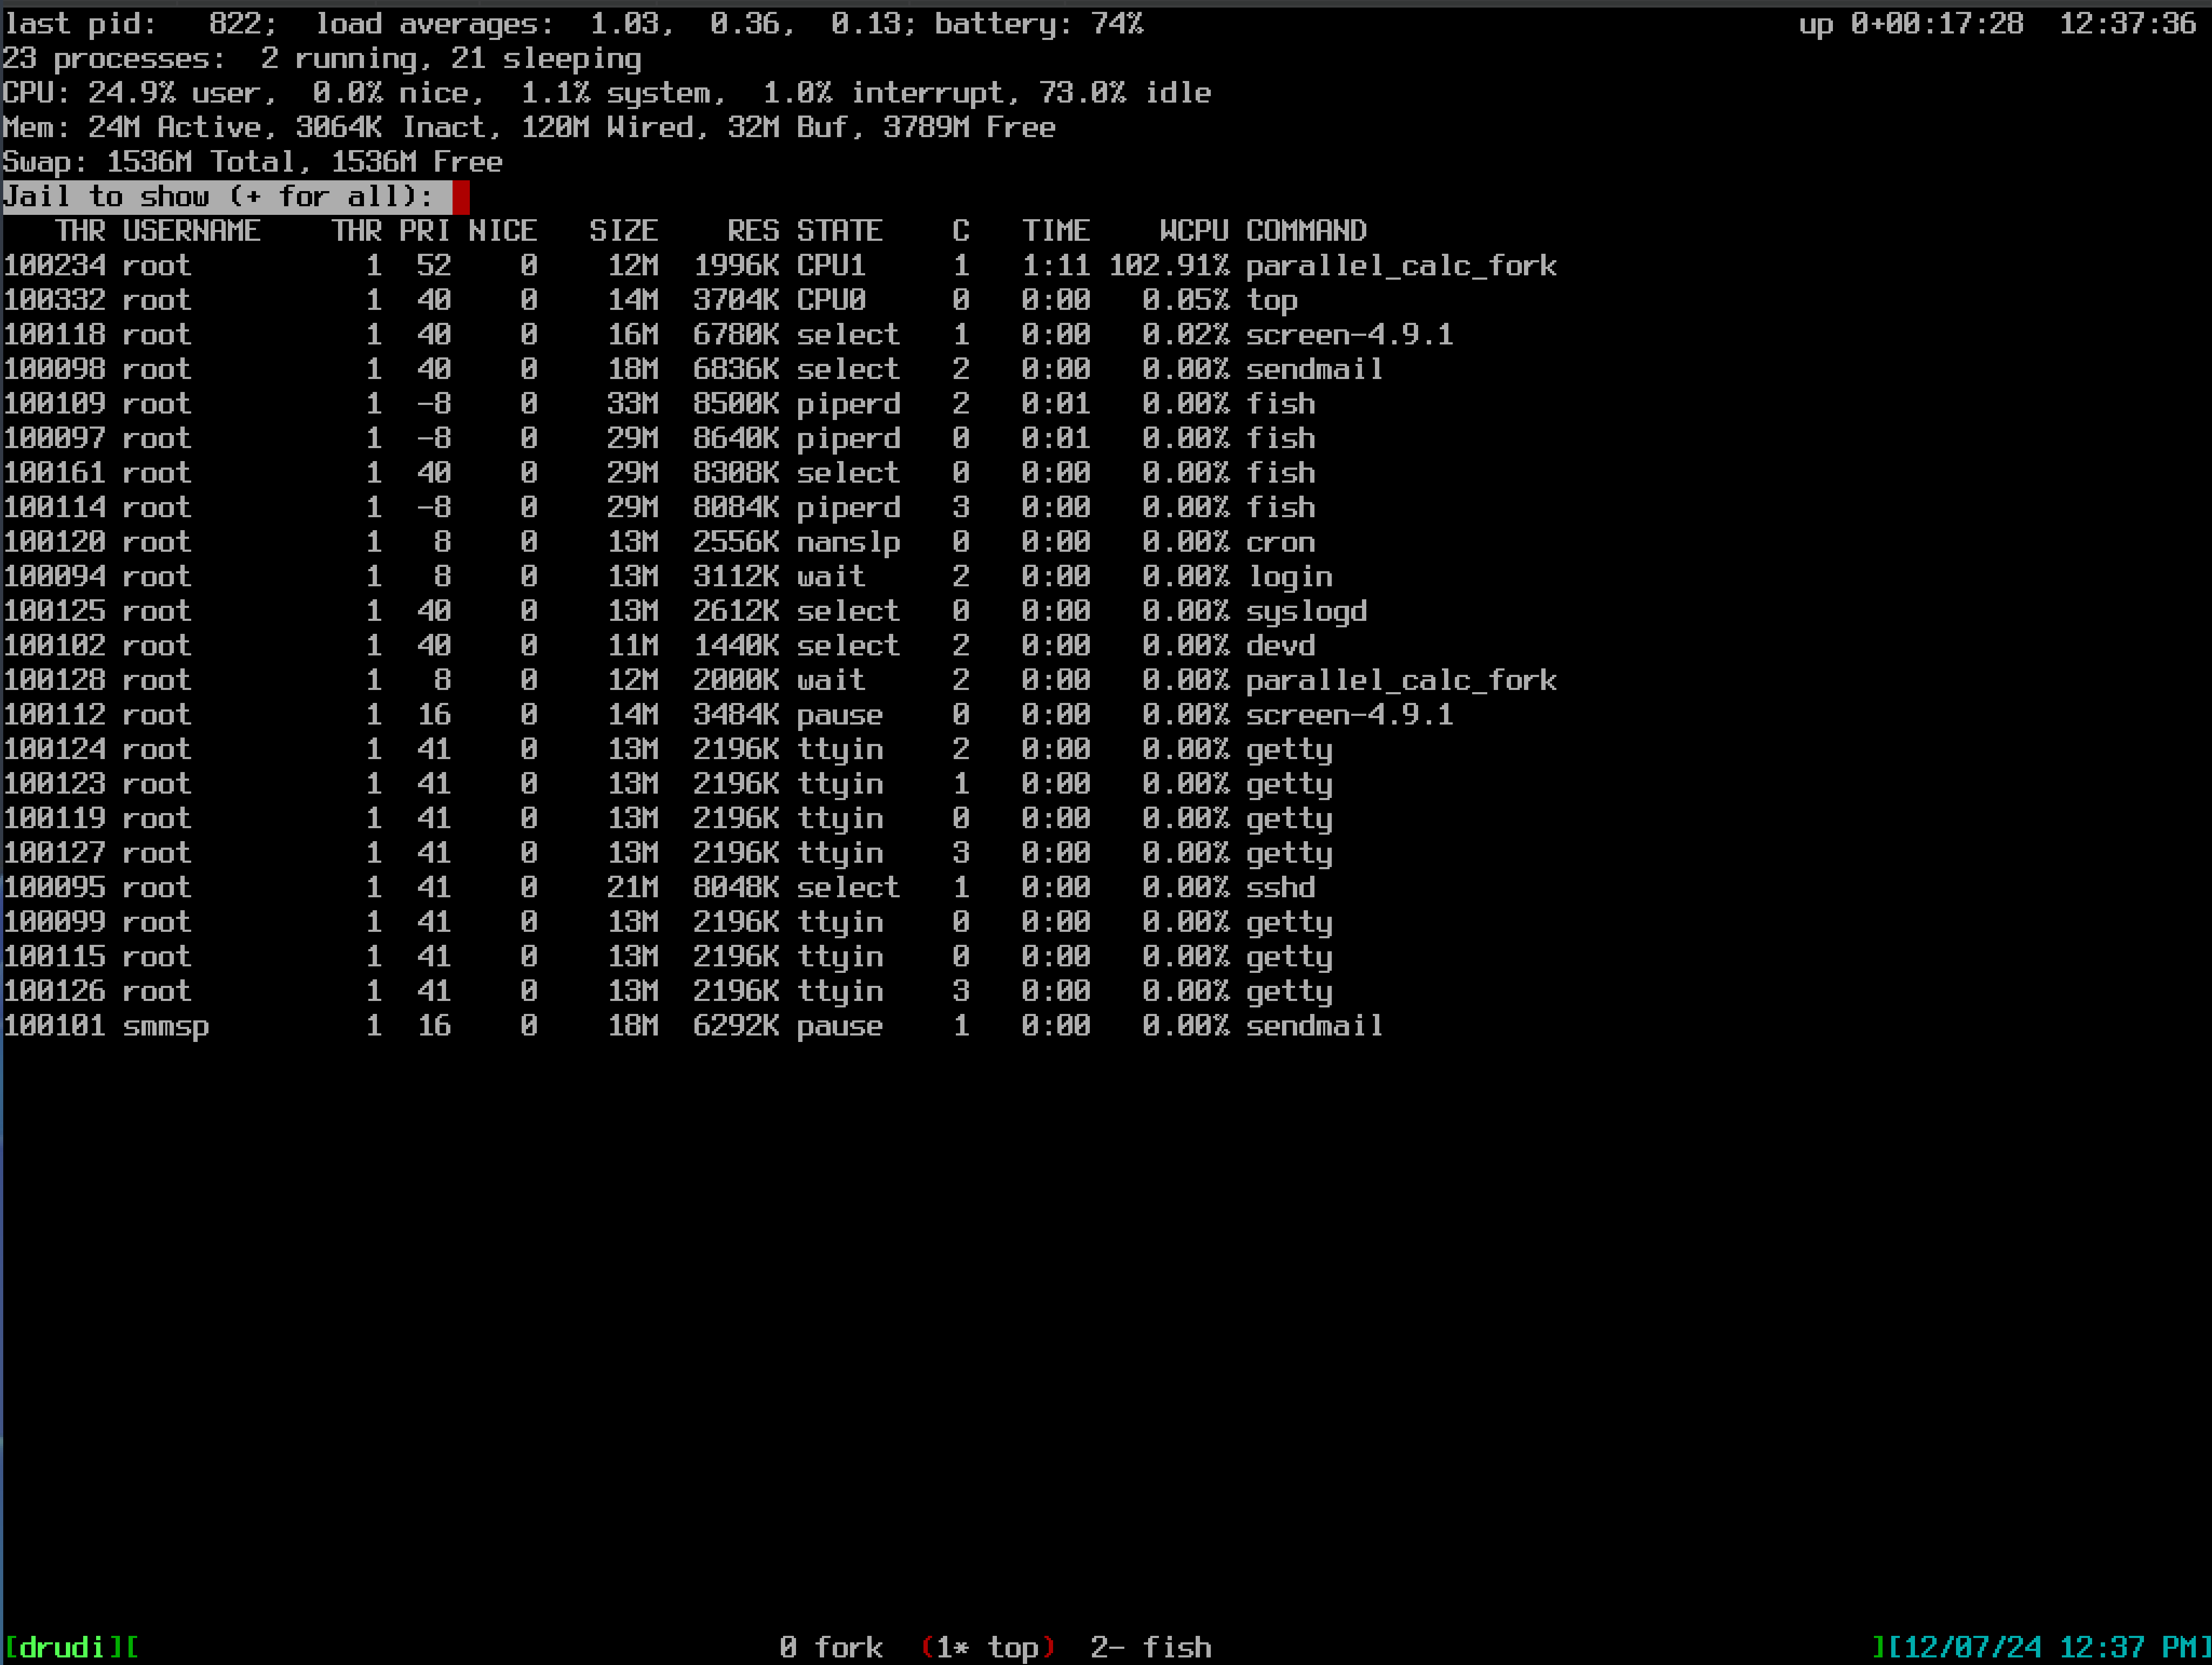
\includegraphics[width=0.5\textwidth]{images/top_disabled.png}
    \caption{Estado de los núcleos con el modulo encendido/apagado habilitado para multiples CPUs.}
    \label{fig:top_disabled}
\end{figure}

\begin{figure}[H]
    \centering
    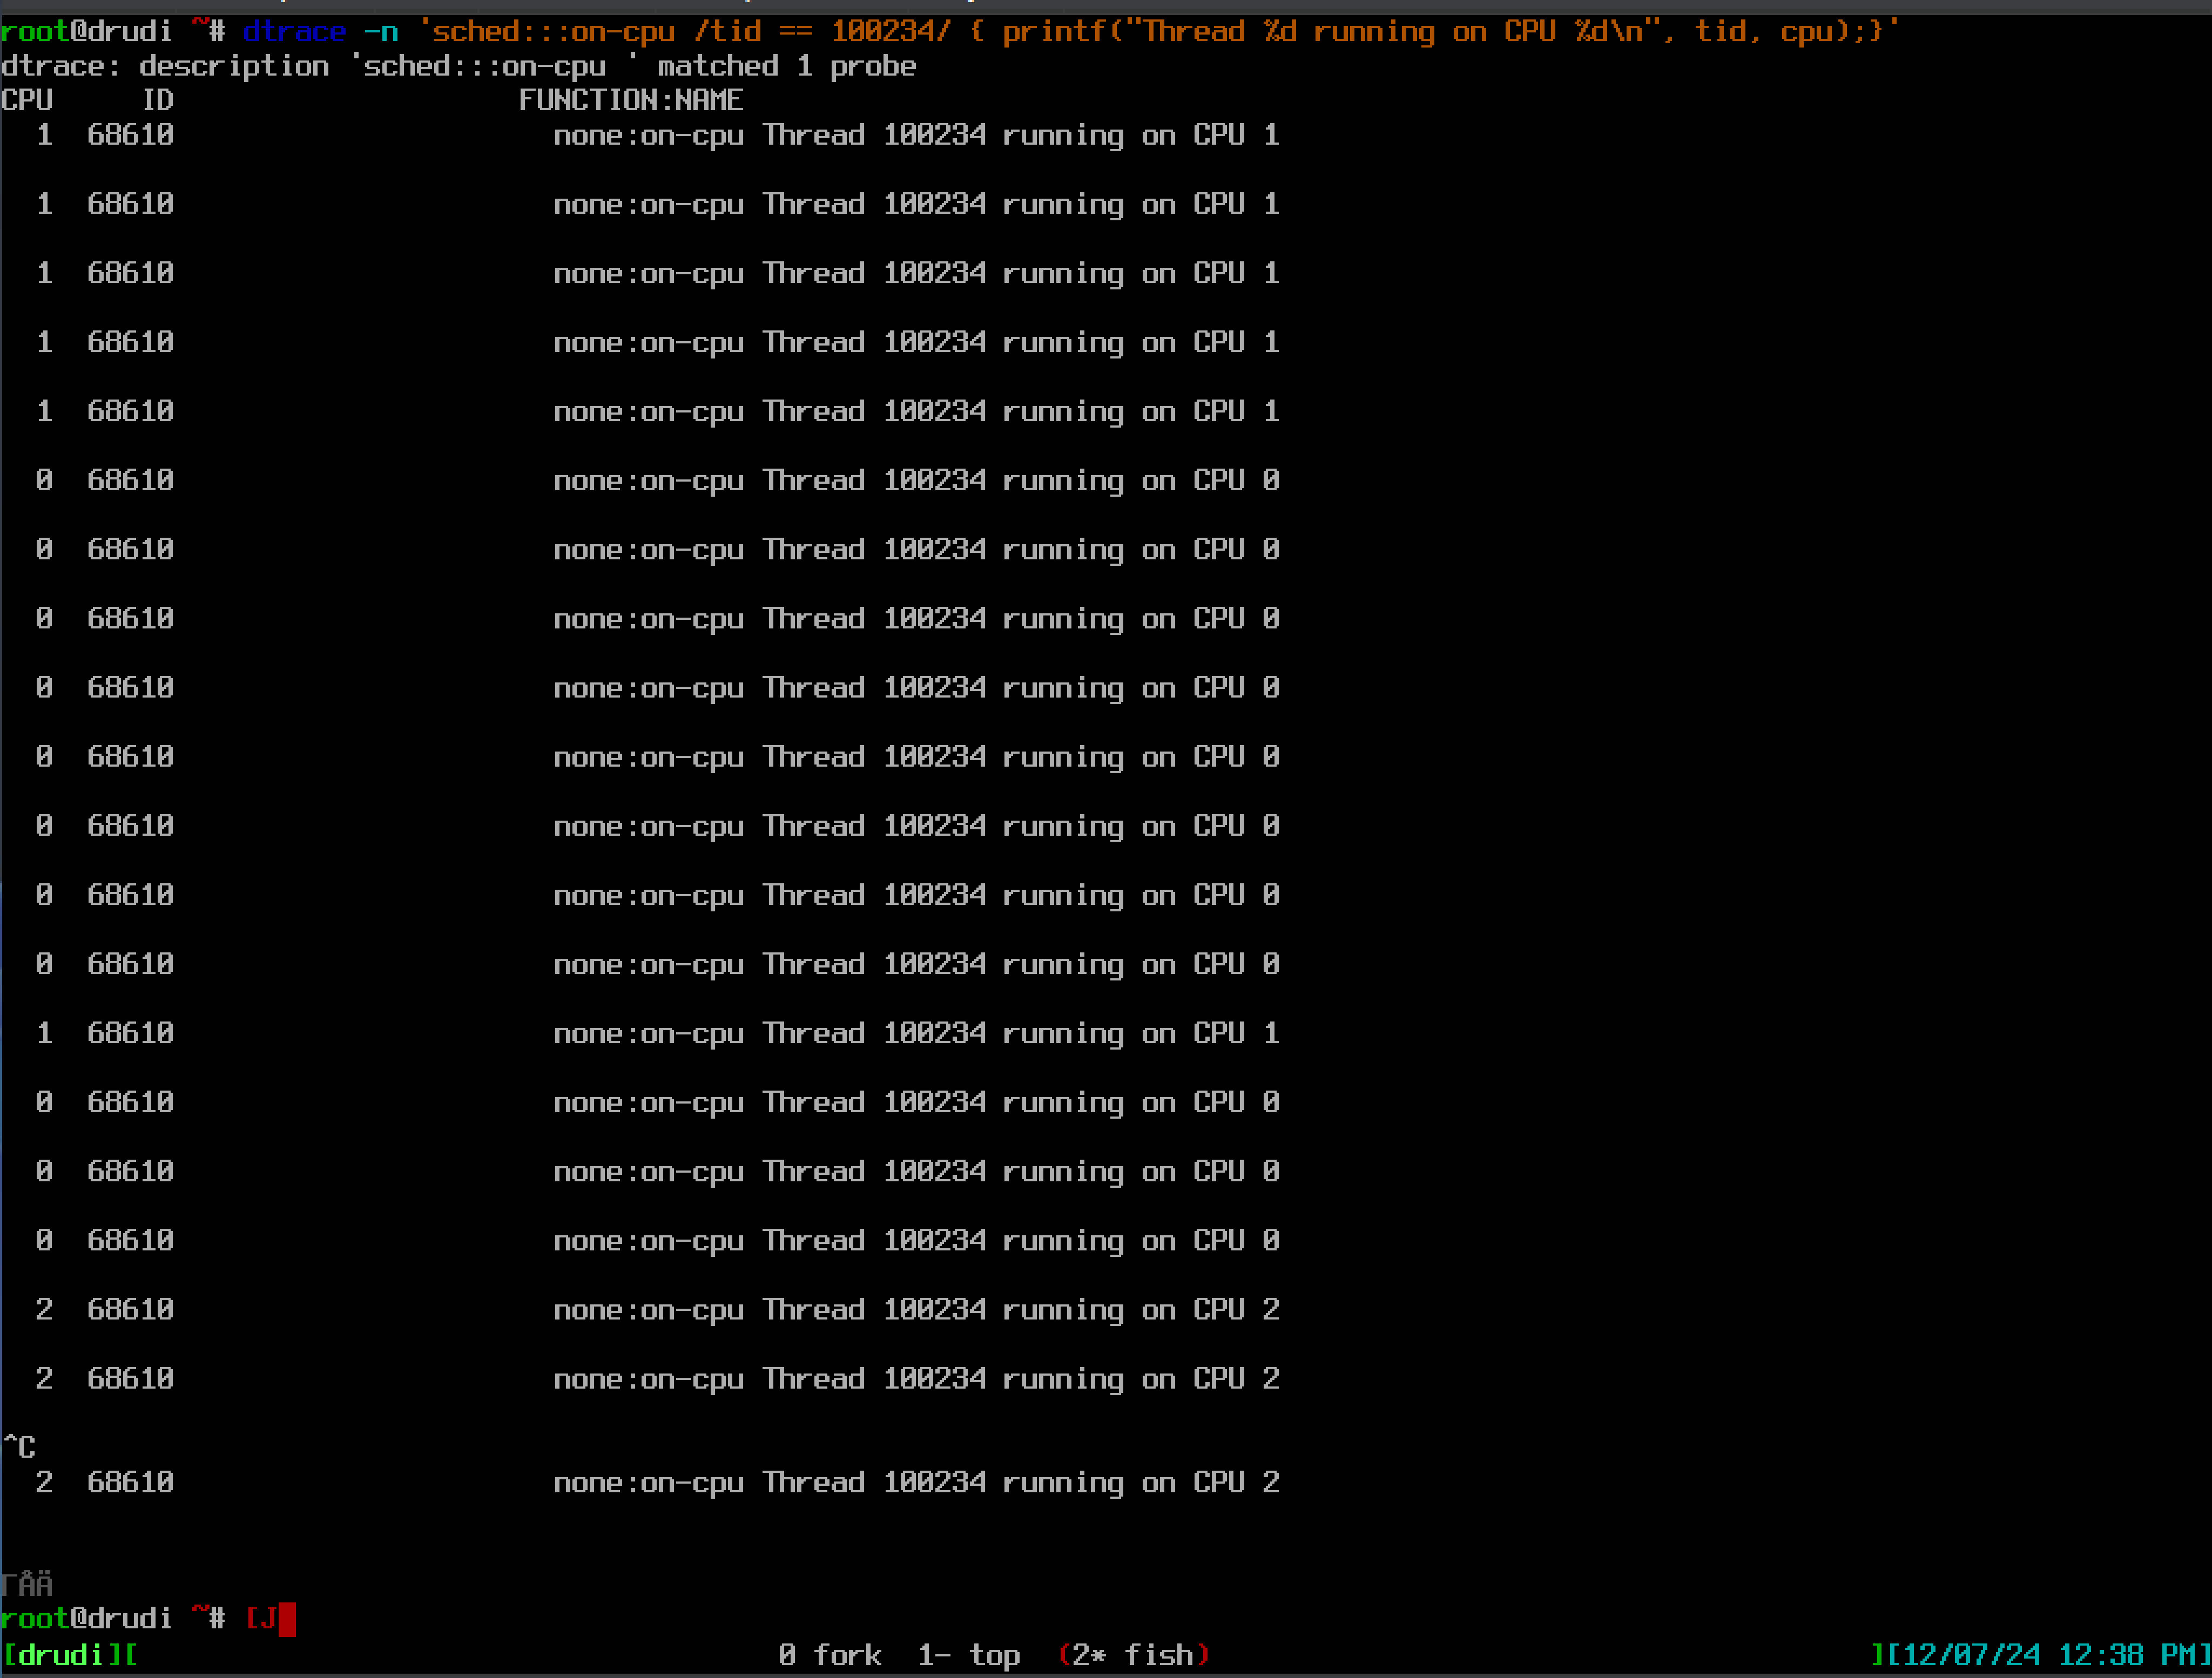
\includegraphics[width=0.5\textwidth]{images/dtrace_disabled.png}
    \caption{Estado de los núcleos con el modulo encendido/apagado habilitado para multiples CPUs.}
    \label{fig:dtrace_disabled}
\end{figure}


\subsubsection{Comportamiento con el Módulo Habilitado}
Habiendo expuesto el comportamiento del sistema en su condición normal, se sienta una base para la posterior comparación con el desempeño del módulo.\par

Siguiendo un procedimiento similar al empleado con el módulo de encendido y apagado, procedimos a ejecutar el programa de estrés, orientado al cálculo de números primos. Durante su ejecución, la herramienta de monitoreo (htop) permite la observación de los distintos subprocesos vinculados a este programa y la información específica de cada uno.\par

Luego de haber activado el módulo podemos observar que los resultados obtenidos concuerdan con la información proporcionada por la  herramienta de monitoreo. Como era de esperar, este subproceso estuvo vinculado al CPU durante toda su ejecución. Además, ningún otro hilo o proceso se ejecutó en ningún momento en este núcleo, evidenciando así su exclusividad y el correcto funcionamiento del desarrollo.\par

\begin{figure}[H]
    \centering
    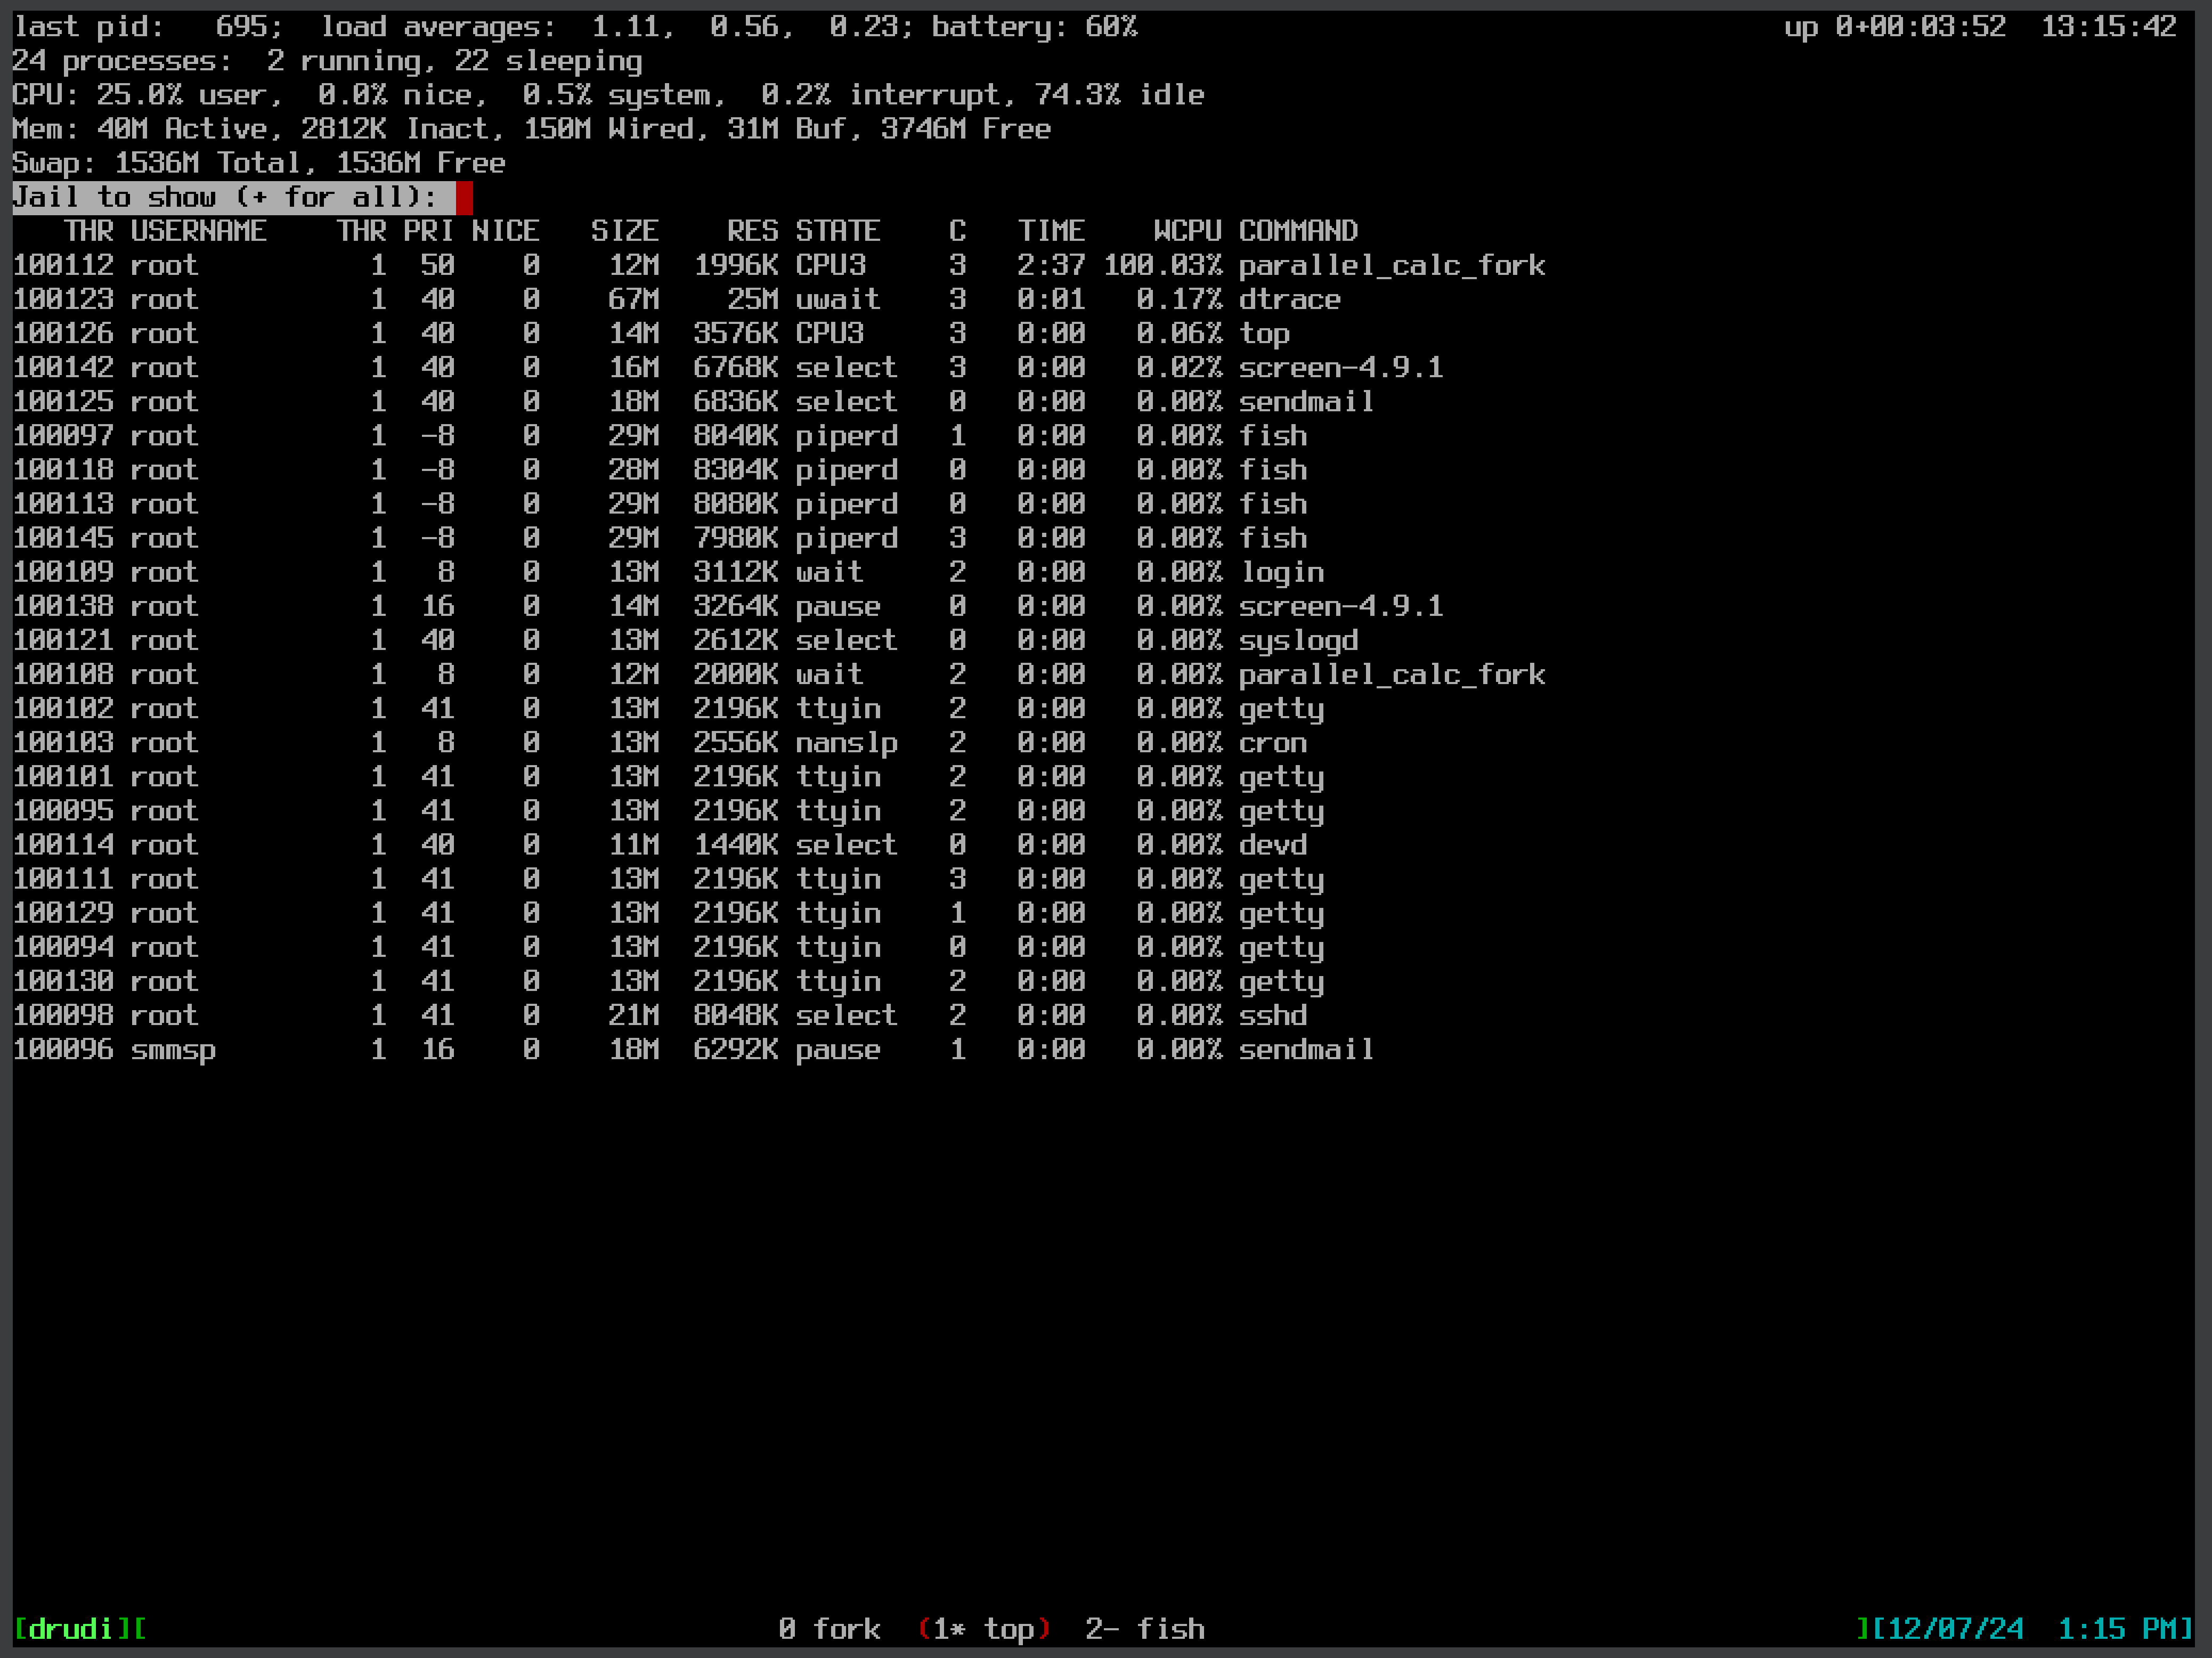
\includegraphics[width=0.5\textwidth]{images/cpuMonopolized-idle.png}
    \caption{Estado de los núcleos con el modulo encendido/apagado habilitado para multiples CPUs.}
    \label{fig:cpuMonopolized-idle}
\end{figure}

\begin{figure}[H]
    \centering
    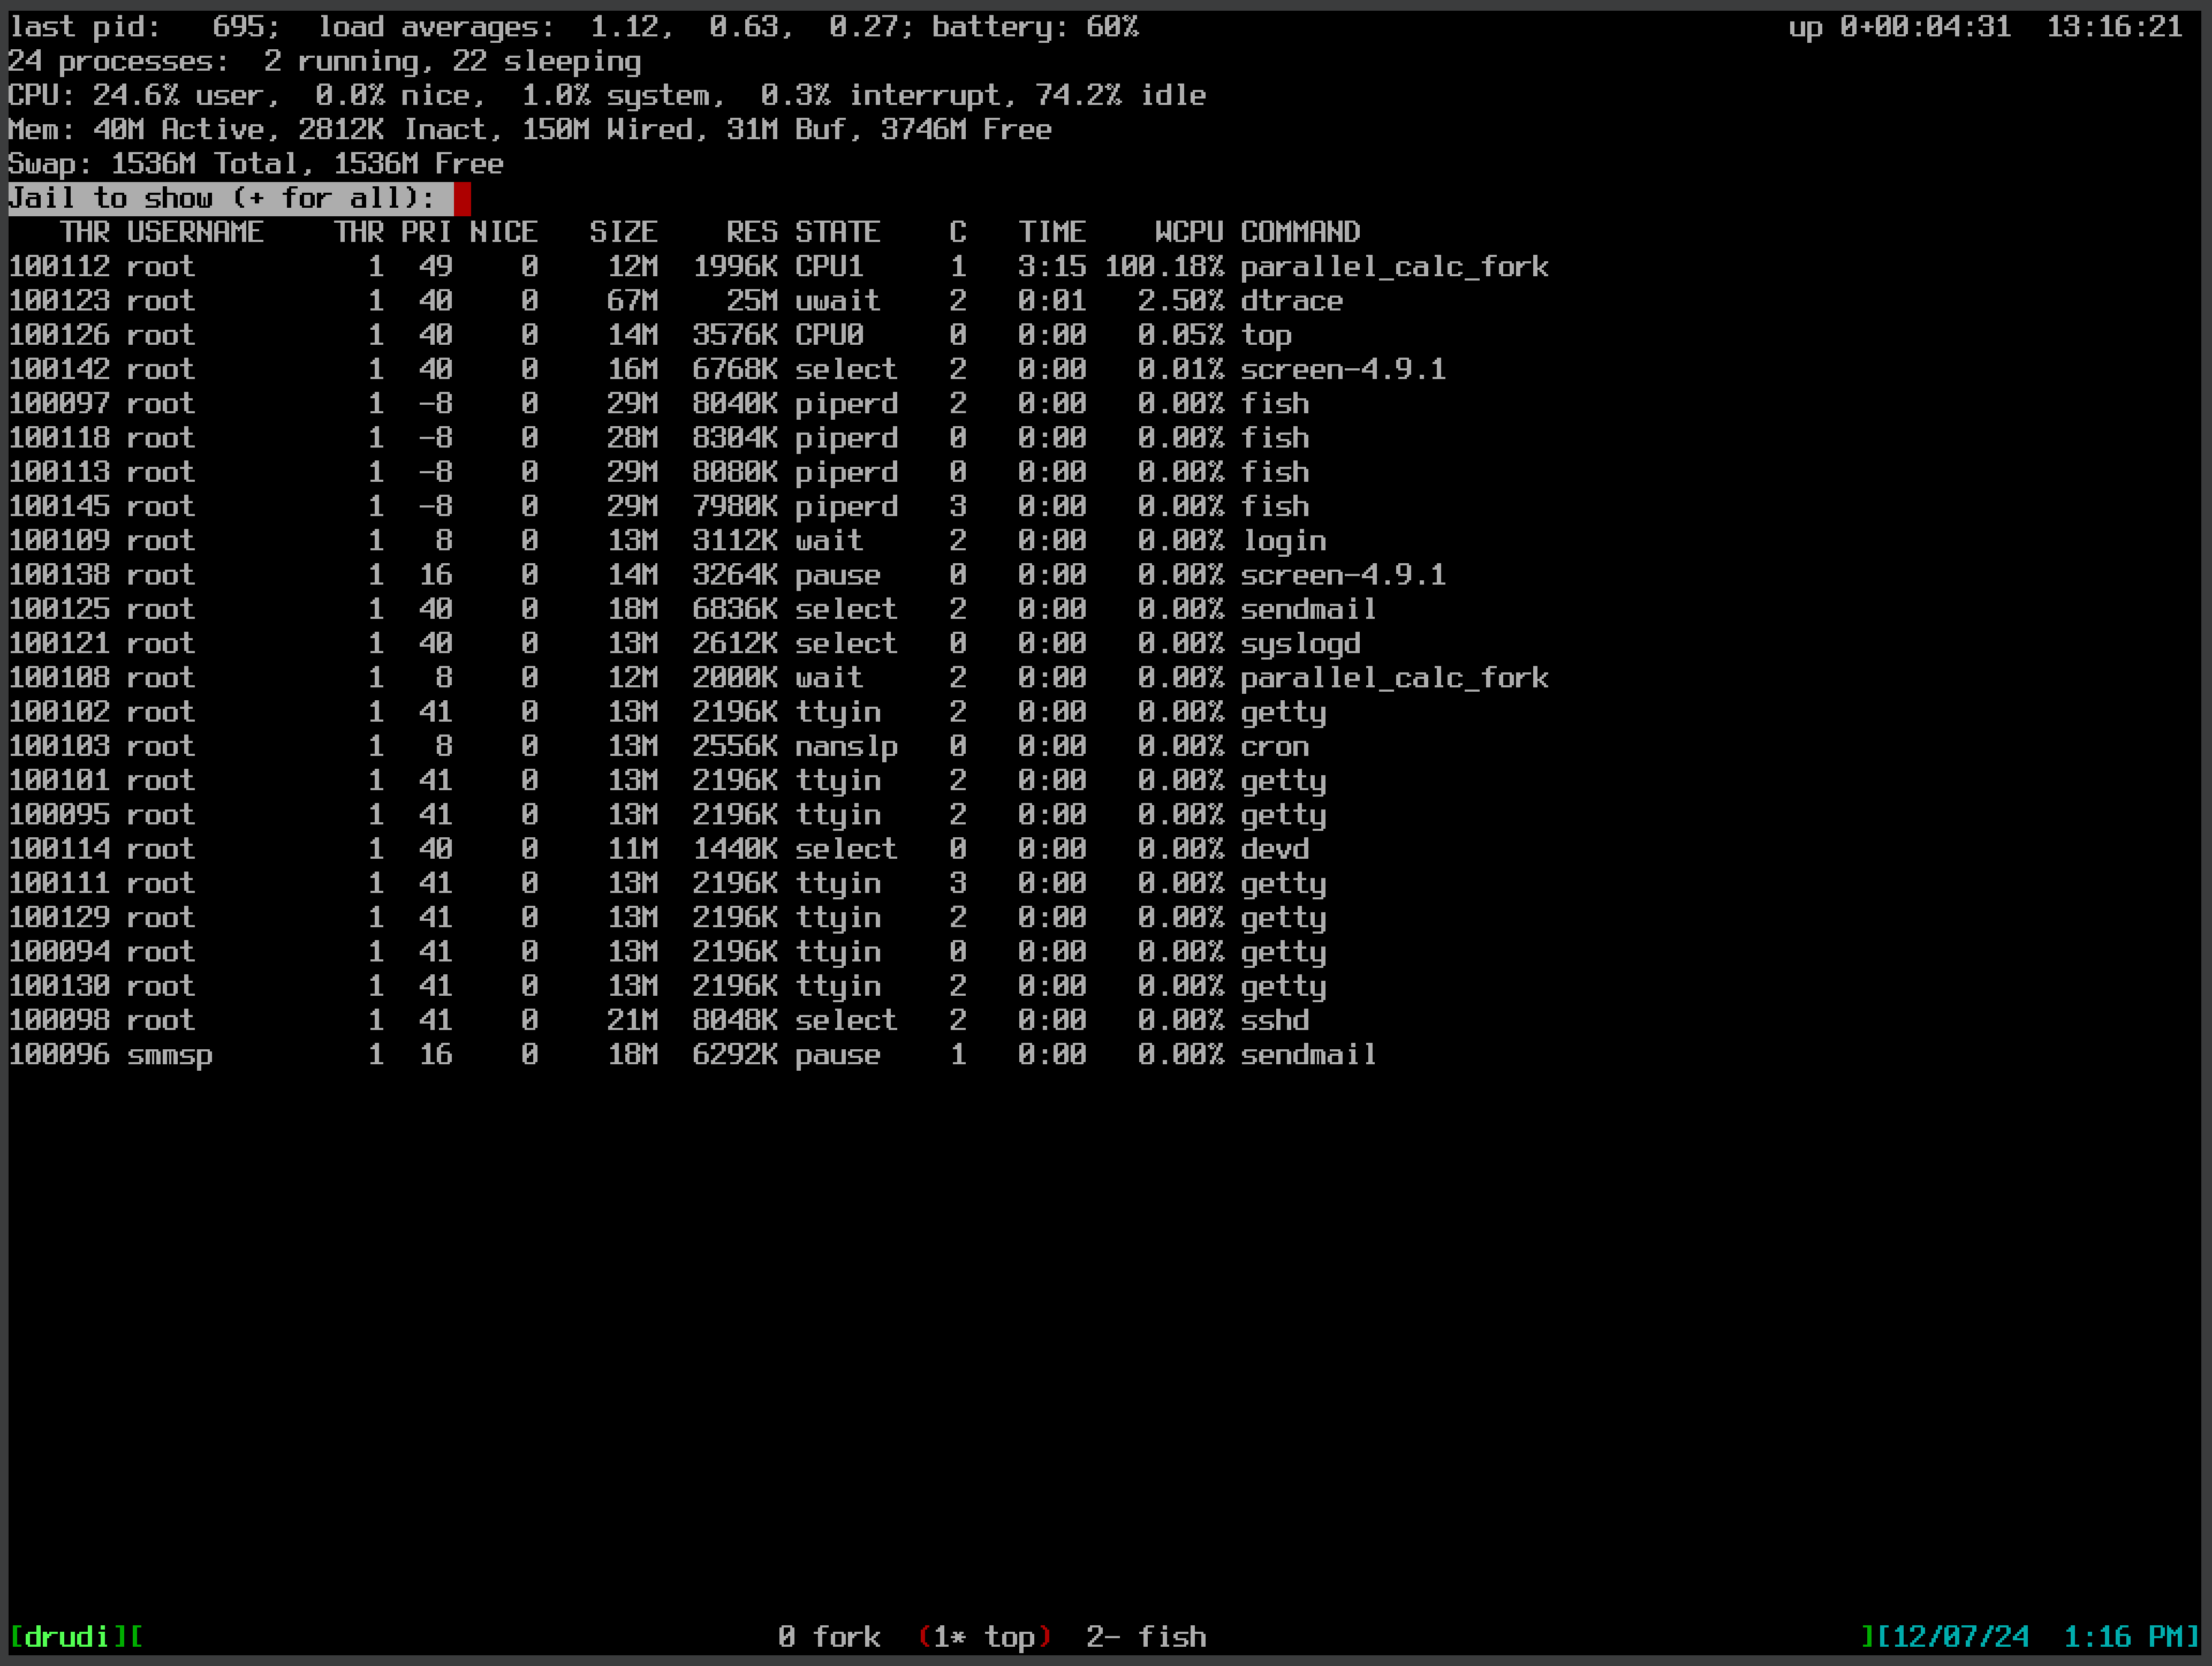
\includegraphics[width=0.5\textwidth]{images/cpuMonopolized-on.png}
    \caption{Estado de los núcleos con el modulo encendido/apagado habilitado para multiples CPUs.}
    \label{fig:cpuMonopolized-on}
\end{figure}

\begin{figure}[H]
    \centering
    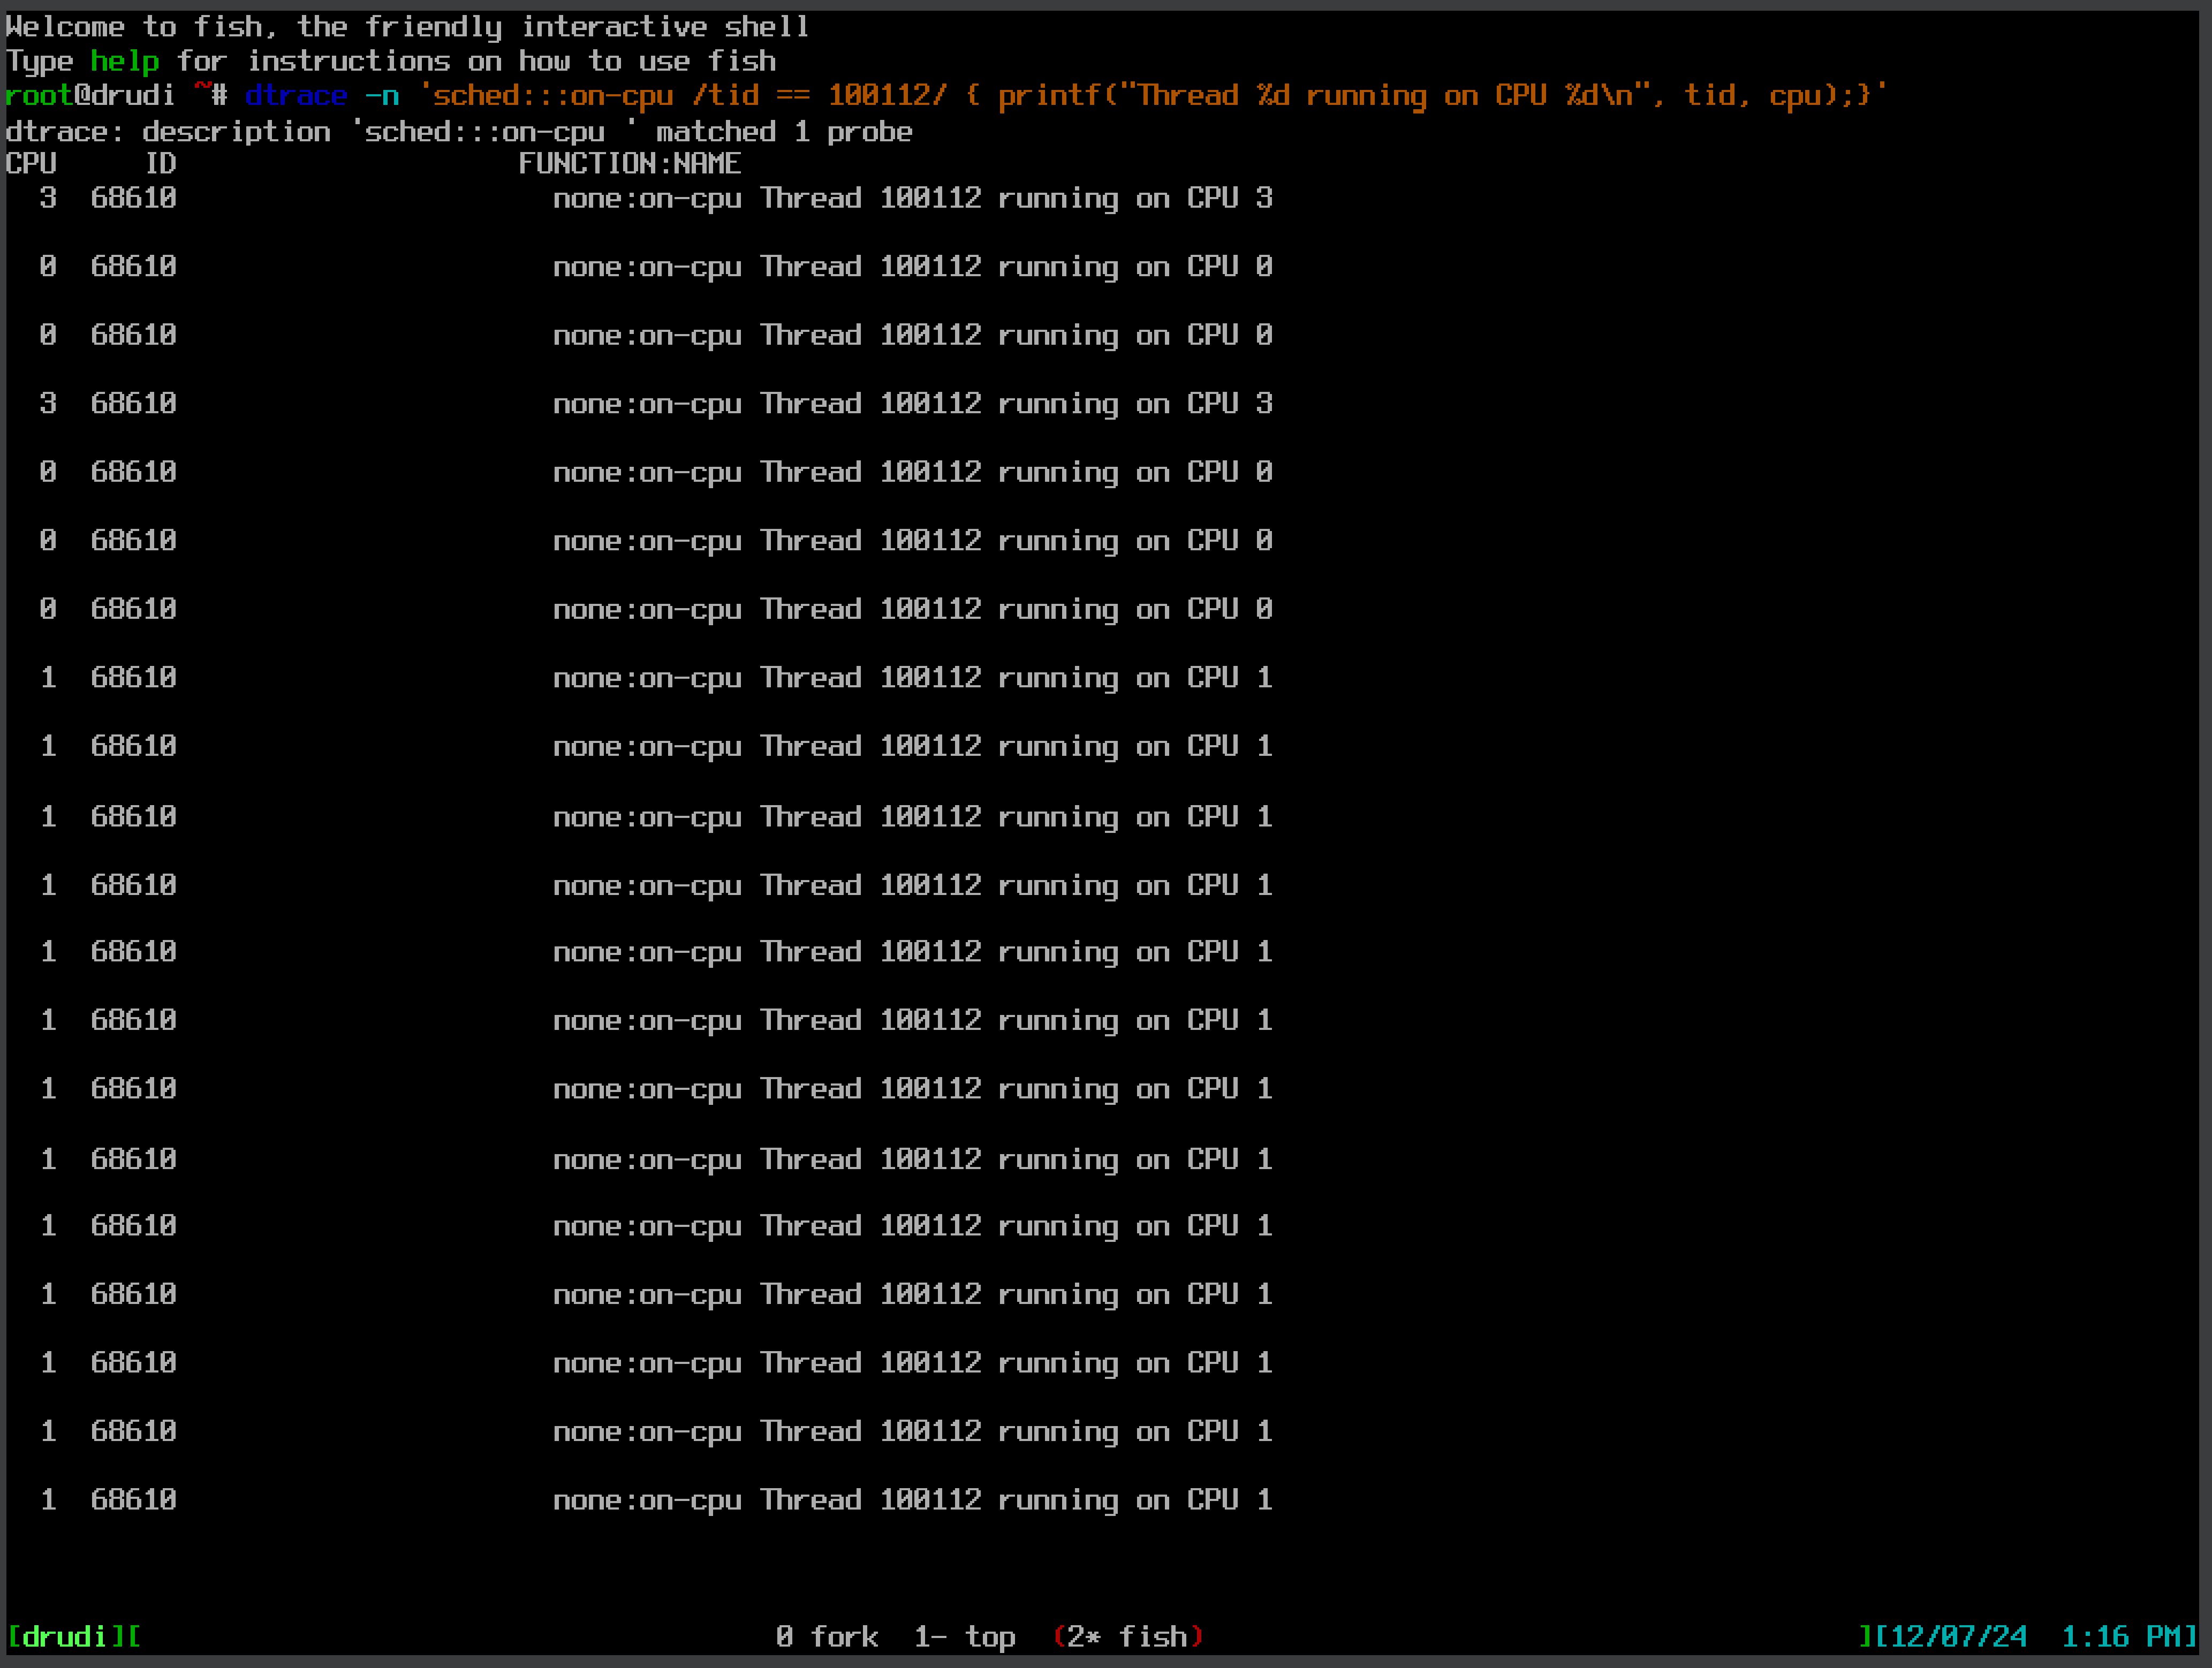
\includegraphics[width=0.5\textwidth]{images/cpuMonopolized-dtrace.png}
    \caption{Estado de los núcleos con el modulo encendido/apagado habilitado para multiples CPUs.}
    \label{fig:cpuMonopolized-dtrace}
\end{figure}



% TODO{Mover a apendice}
% Con el programa en ejecución y el monitoreo activado, el siguiente paso implica la configuración del módulo; en otras palabras, es el momento de actualizar las variables dentro del código del módulo. La primera variable a considerar es el identificador del subproceso que deseamos anclar a un núcleo específico, obtenido previamente del programa de monitoreo. Una vez que tenemos el identificador, procedemos a seleccionar en qué núcleo asociaremos este hilo, compilando y cargando el módulo de kernel adecuado.\par

% TODO{Mover a apendice}
% Los resultados obtenidos concuerdan con la información proporcionada por la  herramienta de monitoreo. En este caso, hemos seleccionado el hilo con el identificador  878172 y la CPU2. Como era de esperar, tras la ejecución del módulo, este subproceso estuvo vinculado al CPU durante toda su ejecución. Además, ningún otro hilo o proceso se ejecutó en ningún momento en este núcleo, evidenciando así su exclusividad y el correcto funcionamiento del desarrollo.\par

% TODO{Imagen con el hilo asociado al núcleo, quizás también podemos tener un link a video para mostrar hasta que termina de ejecutarse, y con la desactivación del módulo para ver como la CPU vuelve a estar disponible para los otros procesos}

Un caso relevante es el estado del sistema una vez que el programa de estrés ha concluido pero el módulo permanece activado. En estas condiciones, se puede observar cómo la CPU al que se había anclado el hilo permanece “reservado”, sin ejecutar ningún hilo que no posea el ID especificado, mientras que los procesos restantes solo se ejecutan en los núcleos liberados. Con esto en mente, se puede identificar una similitud con el funcionamiento del módulo de encendido/apagado al desactivar un núcleo.\par

Al desactivar el módulo, el sistema continúa operando según lo esperado, con todos sus núcleos disponibles, tal como lo haría en su estado normal.


\subsection{Resultados de las actualizaciones en la versión del S.O.}
En esta sección, se expondrán los resultados derivados de las actualizaciones implementadas en el marco del proyecto integrador previo. Es relevante subrayar que estas actualizaciones se llevaron a cabo con el propósito de sincronizar el proyecto con la versión más reciente y estable del sistema operativo (versión 13.1). Dado que la implementación original demostró su eficacia en la versión 11, el énfasis principal en esta sección se dirigirá a garantizar la continuidad de dicho rendimiento.\par

Esta fue la primera tarea abordada en este proyecto, y la elección de priorizarla desde el inicio se fundamentó en la necesidad de mantenerse alineado con la comunidad y acceder a posibles recursos de apoyo cuando fuese necesario. Asimismo, esta estrategia facilitó el desarrollo sobre una base de código más actualizada, evitando conflictos significativos que pudieran surgir en fases finales del desarrollo.\par

A pesar de la necesidad de revisar numerosos conflictos generados entre el código del planificador en la versión 11 y la versión 13 de FreeBSD, los resultados finales obtenidos de esta etapa confirman que la actualización se realizó con éxito. El sistema operativo, con el planificador de redes de Petri, mantuvo la estabilidad y el funcionamiento adecuado en las pruebas realizadas.\par

El código correspondiente a esta etapa se encuentra en una rama específica del repositorio del proyecto. Debido a la estructura de ramas y modalidad de trabajo que se planteó para la realización de este trabajo integrador, también podemos encontrar una rama por cada actualización que se fue realizando progresivamente desde la 11 hasta la 13.1.\par

% TODO{MOSTRAR ALGUNAS IMAGENES DEL PROYECTO CORRIENDO CON LA VERSION 13.1 Y UTILIZANDO LA RED}

% TODO{OPCIONAL - VER SI LO AGREGAMOS}
% \subsection{Resultados del tareas extra}



\chapter{Conclusión y trabajos futuros}

\section{Conclusiones}

El desarrollo de este trabajo permitió confirmar que es posible extender el planificador basado en Redes de Petri en FreeBSD sin modificar su estructura base. La actualización del planificador a la versión 13.1 garantiza su compatibilidad con versiones recientes del sistema operativo y sienta una base para trabajos futuros.\par

Además, la implementación de los módulos de encendido/apagado de procesadores y de monopolización de núcleos mostró que es viable gestionar dinamicamente los recursos del sistema operativo a nivel de software. El hecho de haber incorporado estas funcionalidades sin modificar el núcleo del planificador confirma que es posible extender sus capacidades de manera modular y organizada, aprovechando las ventajas de las Redes de Petri.\par

Sin embargo, el trabajo realizado se centró en la implementación de estos mecanismos sin abordar aún su impacto en la eficiencia del sistema. En particular, el módulo de encendido/apagado de procesadores permite seleccionar qué núcleos estarán activos, pero aún no se ha explorado su integración con mecanismos de hardware que optimicen el consumo energético. Del mismo modo, el módulo de monopolización de núcleos cumple con su propósito de asignar procesadores exclusivos a ciertos hilos, pero su efecto en el rendimiento global del sistema aún requiere mayor análisis.\par

Por otro lado, la interacción con la comunidad y el estudio del código fuente fueron aspectos clave para la resolución de problemas técnicos y demuestran la importancia de seguir de cerca las actualizaciones y cambios en el ecosistema del sistema operativo.\par

\section{Trabajos Futuros}

Mirando hacia el futuro, nuestra implementación proporciona una base sólida para investigaciones adicionales y mejoras continuas. Identificamos varias áreas en las que se podrían realizar avances significativos.\par

\subsection{Automatización de la Activación de los Módulos}
Hasta el momento, la activación o desactivación de los módulos se realiza de forma manual. Una posible mejora futura es la integración de un mecanismo automático basado en \textit{triggers} dentro del sistema operativo, permitiendo que la Red de Petri active o desactive los módulos en función de la carga de trabajo del sistema.\par

\subsection{Integración con Hardware para Optimización Energética}
Si bien el módulo de encendido/apagado de procesadores permite seleccionar qué núcleos estarán inactivos, actualmente su implementación se encuentra limitada a una gestión a nivel de software. Un siguiente paso clave sería explorar cómo estas decisiones pueden traducirse en una reducción efectiva del consumo energético a nivel de hardware, aprovechando mecanismos de administración de energía soportados por los procesadores modernos.\par

\subsection{Solución definitiva al fallo de página con la placa de red encendida}
Como se comentó en la sección \ref{ch:problema_red} del presente informe, actualmente tenemos problemas en el uso regular del sistema operativo cuando la placa de red se encuentra encendida. Si bien es una falla que se puede detectar también en la versión del proyecto integrador previo, consideramos que es un punto importante a tener en cuenta para mejorar la experiencia de trabajo sobre este proyecto.\par

\subsection{Optimización del \textit{timeslice} para procesadores apagados}
Otra posible mejora para futuras versiones del sistema es la optimización de la gestión del \textit{timeslice} asignado a los hilos, permitiendo un manejo más eficiente del tiempo de ejecución. En el caso del módulo de encendido/apagado de procesadores, esta optimización reduciría la cantidad de operaciones de encolado y desencolado del \textit{idlethread}, evitando procesos innecesarios y disminuyendo la sobrecarga del sistema. Para el módulo de monopolización de núcleos, ajustar dinámicamente el \textit{timeslice} permitiría que los hilos anclados se ejecuten por períodos más largos sin interrupciones innecesarias. Esto evitaría, al planificador, algunos cambios de contexto y haría más predecible la ejecución de estos procesos sin afectar la estabilidad del sistema.\par

\subsection{Implementación de Políticas de Afinidad mediante la Red}
Actualmente, FreeBSD dispone de métodos nativos para gestionar la afinidad entre hilos y procesadores. Sin embargo, la migración de esta implementación hacia el enfoque basado en Redes de Petri permitiría un control más centralizado de la asignación de recursos.\par

En resumen, el trabajo realizado representa un primer paso hacia una planificación más flexible y modular en sistemas operativos. Los próximos avances deberán centrarse en traducir estas mejoras en beneficios concretos en términos de eficiencia energética, rendimiento y automatización del sistema.\par

% \begin{thebibliography}{9}
%     \bibitem{bib1} Tomás Turina, Nicolás Papp. (2019). \textit{Modelado del planificador a corto plazo con redes de Petri}.
%     \bibitem{bib2} Marshall Kirk McKusick, George V. Neville-Neil, Robert N.M. Watson. (2014). \textit{The Design and Implementation of the FreeBSD Operating System (2nd Edition)}.
%     \bibitem{bib3} Marshall Kirk McKusick, Keith Bostic, Michael J. Karels, John S. Quarterman. (1996). \textit{The Design and Implementation of the 4.4BSD Operating System}.
%     \bibitem{bib4} Marshall Kirk McKusick. (2020). \textit{An Overview of Scheduling in the FreeBSD Kernel}.
%     \bibitem{bib5} Stanford Secure Computer Systems (2010). \textit{4.4BSD Scheduler}. % (https://www.scs.stanford.edu/23wi-cs212/pintos/pintos_7.html)
% \end{thebibliography}


\bibliographystyle{plain}
\bibliography{references}
\appendix

\section{Apéndice 1: Archivos de diferencias}\label{appendix:apA}

\subsection{\textit{sched\_switch} (v12 a v13): Firma de la función y variables}\label{appendix:apA1}

\begin{lstlisting}[language=diff]
- void sched_switch(struct thread *td, struct thread *newtd, int flags)
+ void sched_switch(struct thread *td, int flags)
{
+   struct thread *newtd;
    struct mtx *tmtx;
    struct td_sched *ts;
    struct proc *p;
    int preempted;

-   tmtx = NULL;
+   tmtx = &sched_lock;
    ts = td_get_sched(td);
    p = td->td_proc;

    THREAD_LOCK_ASSERT(td, MA_OWNED);
...
}
\end{lstlisting}



\subsection{\textit{sched\_switch} (v12 a v13): Cambio de posición del bloque que bloquea el hilo previo al \textit{resource\_expulse\_thread}}\label{appendix:apA2}

\begin{lstlisting}[language=diff]
+   if (td->td_lock != &sched_lock) {
+   	mtx_lock_spin(&sched_lock);
+   	tmtx = thread_lock_block(td);
+   	mtx_unlock_spin(tmtx);
+   }

   if ((td->td_flags & TDF_NOLOAD) == 0)
   	sched_load_rem();

    td->td_lastcpu = td->td_oncpu;
    preempted = (td->td_flags & TDF_SLICEEND) == 0 && (flags & SW_PREEMPT) != 0;
    td->td_flags &= ~(TDF_NEEDRESCHED | TDF_SLICEEND);
    td->td_owepreempt = 0;
    td->td_oncpu = NOCPU;

    resource_expulse_thread(td, flags);

-   if (td->td_lock != &sched_lock) {
-   	mtx_lock_spin(&sched_lock);
-   	tmtx = thread_lock_block(td);
-   	mtx_unlock_spin(tmtx);
-   }
...
\end{lstlisting}


\subsection{\textit{sched\_switch} (v12 a v13): Selección y ejecución de un nuevo thread}\label{appendix:apA3}

\begin{lstlisting}[language=diff]
+   newtd = choosethread();
-   if (newtd) {
-       /*
-        * The thread we are about to run needs to be counted
-        * as if it had been added to the run queue and selected.
-        * It came from:
-        * * A preemption
-        * * An upcall
-        * * A followon
-        */
-       KASSERT((newtd->td_inhibitors == 0),
-           ("trying to run inhibited thread"));
-       newtd->td_flags |= TDF_DIDRUN;
-           TD_SET_RUNNING(newtd);
-       if ((newtd->td_flags & TDF_NOLOAD) == 0)
-           sched_load_add();
-       if (ts->ts_runq != &runq){
-           resource_fire_net(newtd, TRAN_UNQUEUE + (PCPU_GET(cpuid)*CPU_BASE_TRANSITIONS));
-       }
-       else{
-           resource_fire_net(newtd, TRAN_FROM_GLOBAL_CPU + (PCPU_GET(cpuid)*CPU_BASE_TRANSITIONS));
-       }
-   } else {
-       newtd = choosethread();
-       MPASS(newtd->td_lock == &sched_lock);
-   }

    resource_execute_thread(newtd, PCPU_GET(cpuid));

\end{lstlisting}

% TODO: ANEXO
\section{Apéndice 2: Detalles de la implementación del módulo de monopolizado}\label{appendix:apB}

El planificador 4BSD maneja los cambios de contexto cuando un hilo termina su ejecución o queda bloqueado, generando una interrupción para seleccionar un nuevo hilo. La función principal para gestionar estos cambios es \textit{mi\_switch()}, que invoca \textit{sched\_switch()}. Esta función se encarga de preparar el nuevo hilo para su ejecución y usa \textit{sched\_add()} para añadirlo a la cola de un procesador, considerando la afinidad y las políticas del planificador. Luego, \textit{sched\_choose()} selecciona el hilo a ejecutar y realiza el cambio de contexto si es necesario.

% Para integrar el módulo de monopolización, modificamos \textit{sched\_add()} para permitir que ciertos hilos se fijen a CPUs específicas. Esto asegura que un CPU ejecute siempre el mismo hilo hasta que se decida lo contrario. Implementamos un arreglo llamado \textit{pinned\_threads\_per\_cpu}, que almacena el ID del hilo asignado a cada CPU. Si un CPU está libre, el valor correspondiente en el arreglo es -1. Este ajuste facilita la asignación precisa de hilos a CPUs y asegura que cada procesador ejecute los hilos de manera eficiente según las políticas establecidas.

% En el siguiente ejemplo, se detalla un caso en el que el hilo con ID 100101 tomó control sobre el CPU1 y donde el resto de los procesadores se encuentran funcionando normalmente.

% int \textit{pinned\_threads\_per\_cpu}[CPU\_NUMBER] = \{ -1, 100101, -1, -1 \};

% Al momento de encolar el hilo, se busca cuál de los procesadores disponibles sería la mejor opción para continuar la ejecución del mismo. Ésta decisión se toma dentro del método resource\_choose\_cpu desarrollado en el trabajo integrador previo y extendido actualmente, para hacer uso de este nuevo arreglo de hilos asociados a procesadores. Recibe como parámetro el hilo que se encuentra a encolar, y cuenta con tres condicionales que determinarán dicho procesador:

% \begin{itemize}
%     \item Como primera condición, si el hilo se encuentra dentro del arreglo de \textit{pinned\_threads\_per\_cpu} ya estamos en condiciones de elegir dicho procesador como el indicado para el encolado.
%     \item Si el hilo no se encuentra dentro del arreglo, se intenta asignar a la cola del último procesador en el que se ejecutó. Esto es posible solo si la transición TRAN\_ADDTOQUEUE de dicho procesador se encuentra sensibilizada y el procesador no está monopolizado por otro hilo.
%     \item Por último, si no se cumplen ninguna de las dos condiciones previas, se recorren los diferentes núcleos del procesador y se retorna el primero que cumpla las condiciones necesarias para el encolado.
% \end{itemize}

% Como parte del desarrollo del módulo, también se implementaron algunos métodos complementarios encargados de manejar el estado del arreglo  \textit{pinned\_threads\_per\_cpu}.

% \begin{itemize}
%     \item toggle\_pin\_thread\_to\_cpu: Método encargado de conmutar el estado de monopolización de un procesador. Recibe el ID de un hilo y de un procesador como parámetros y realiza diferentes operaciones de acuerdo al estado del arreglo:
%     \begin{itemize}
%         \item Si el procesador se encuentra libre, se agrega el ID del hilo a la posición correspondiente en el arreglo.
%         \item Si el procesador ya estaba monopolizado por otro hilo, se sobreescribe con el nuevo ID.
%         \item En caso de que el hilo ya se encuentre monopolizando al procesador, lo libera escribiendo el valor -1 en la posición correspondiente.
%     \end{itemize}
%     \item cpu\_available\_for\_thread: Método utilizado por resource\_choose\_cpu para saber si un hilo puede utilizar un procesador, o si este se encuentra monopolizado por otro. Recibe el ID de un hilo y de un procesador como parámetros y retorna 1 en caso de que el procesador se encuentre habilitado para encolar dicho hilo; retorna 0 en caso de que dicho procesador se encuentre tomado por otro hilo.
%     \item get\_monopolized\_cpu\_by\_thread\_id: Método utilizado por resource\_choose\_cpu para obtener el ID del procesador al que se encuentra asociado el hilo enviado por parámetro. Retorna -1 en caso de que no esté anclado a ningún CPU.
% \end{itemize}








\end{document}

\backmatter

\end{document}
